\chapter{PLLによるZRFの自動追従回路}
\section{原理}
\subsection{PLLの伝達特性}
2.1節においては,MR-WPTの周波数特性について解析し,電源から見たMR-WPT回路のリアクタンスが零になる周波数(Zero Reactance Frequency : ZRF)を追従することが,大電力の伝送に有用であることを述べた.この追従動作の実現のために,文献\cite{Fujita2019a}においては,位相同期ループ(Phase Locked Loop : PLL)を用いた回路を提案した.以下,その原理について述べる.\par 

\begin{figure}[b]
\begin{center}

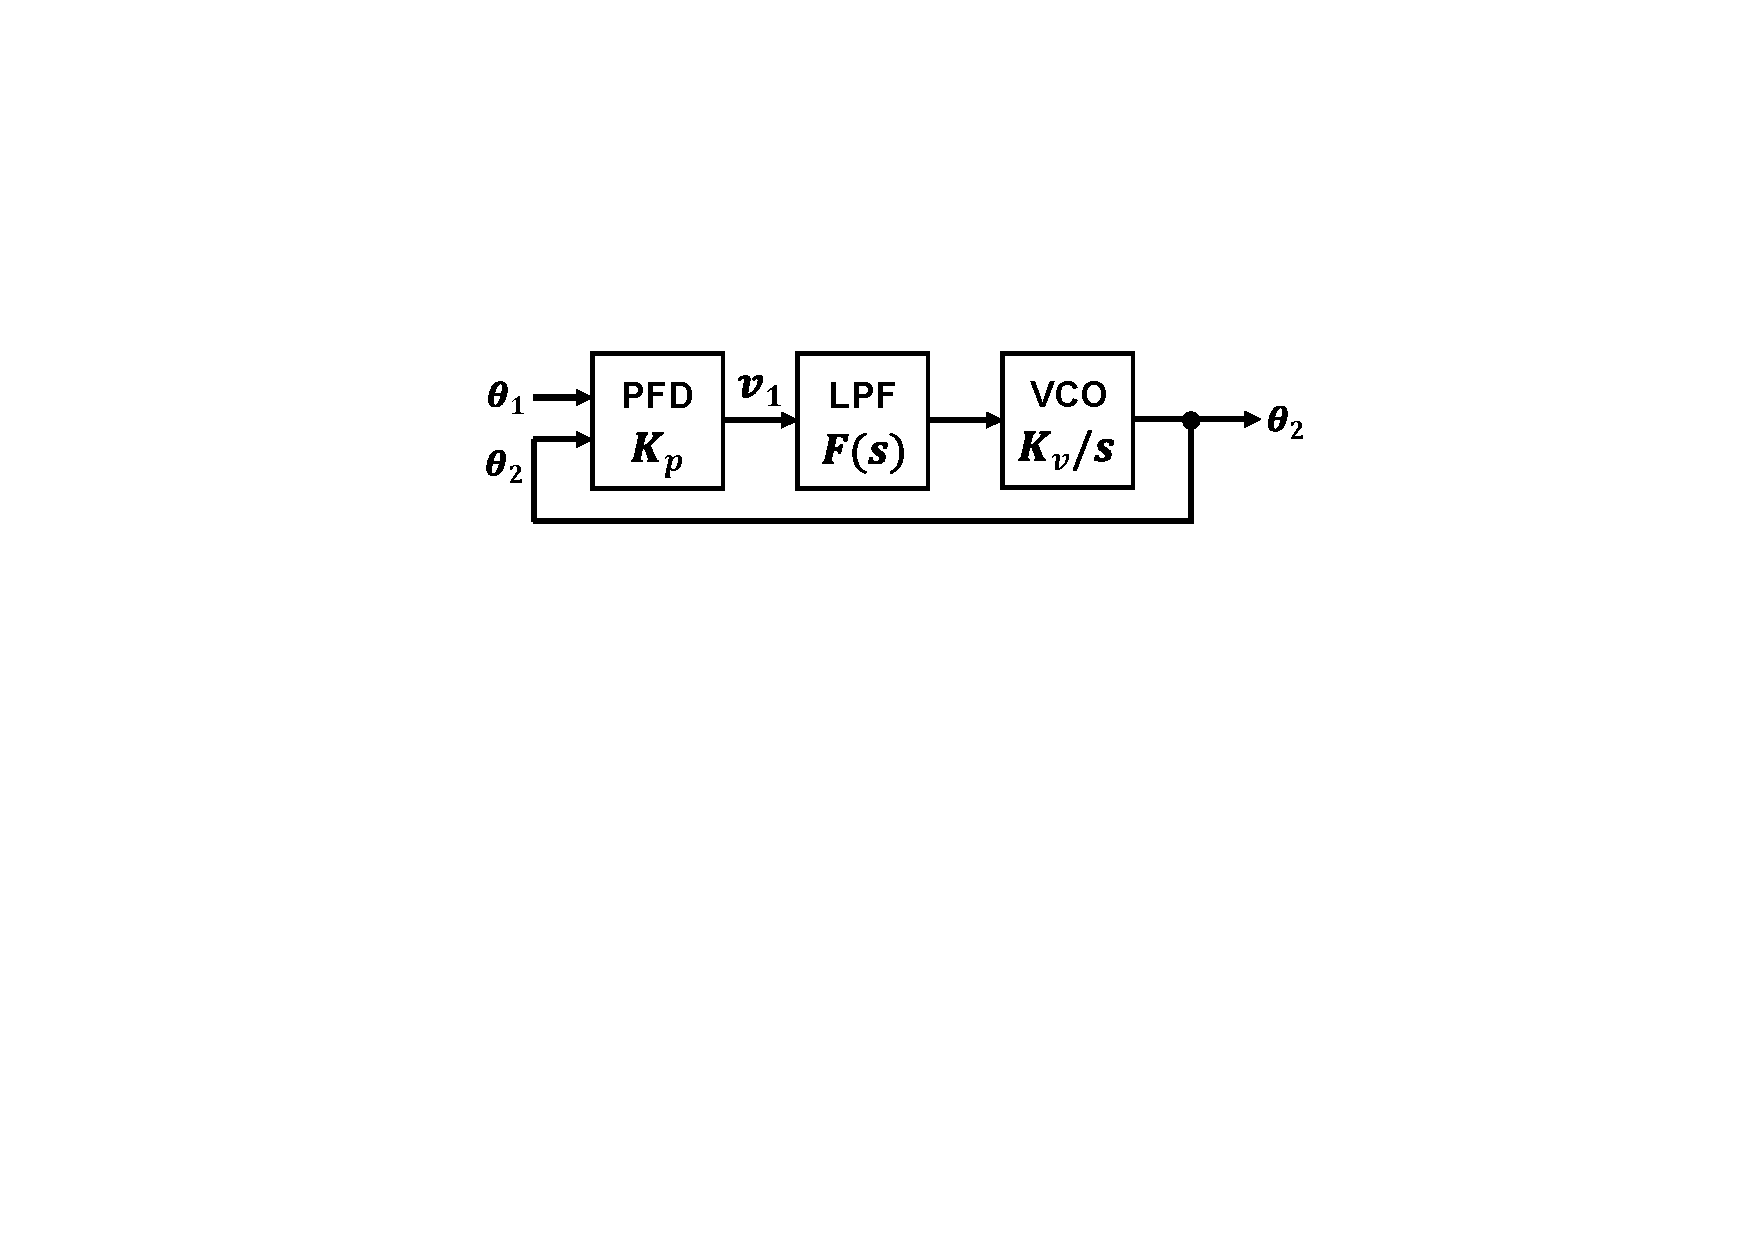
\includegraphics[width=100mm]{figures/pll.pdf}
\caption{PLLの伝達関数モデル}
\label{pll}
\end{center}

\end{figure}

図\ref{pll}に,位相周波数比較器(Phase Frequency Detector : PFD),ループフィルタ(LPF),電圧制御発振器(Voltage Controlled Oscillator : VCO)から成るPLLの伝達関数モデルを示す.同図においては,位相$\theta_1$,$\theta_2$がそれぞれ入出力であり,$K_{p}$はPFDの利得係数,$F(s )$はループフィルタの伝達関数,$K_v$はVCOの利得係数である.PFDは,本来は入出力の位相差$\theta_1-\theta_2$に応じた幅のパルスを出力する回路であるが,ここでは簡単のため,位相差に比例した電圧$v_1$を出力する比例要素として扱う.利得係数$K_p$は,位相差に対してどれだけの電圧を出力するか示すものであるから,次元は$\mathrm{[V/rad]}$である.また,VCOも本来は非線形の要素を含むものであるが,ここでは入力電圧に比例した角周波数を出力する比例要素として扱う.VCOの利得係数の単位は,$\mathrm{[rad/s/V]}$である.\par 
図\ref{pll}に示した伝達関数モデルの閉ループ伝達関数$H(s)$は,

\begin{equation}
H(s) \equiv \frac{\theta_2}{\theta_1}=\frac{K_v K_p F(s)}{s+K_v K_p F(s)}=\frac{1}{1+\frac{s}{K_v K_p F(s)}}
\end{equation}

で与えられる.いま,簡単のためループフィルタの伝達関数$F(s)=1$として,$K_p$と$K_v$の積で与えられるループ利得が十分大きい($K_pK_v \gg 1$)と仮定すれば,$H(s) \simeq 1$となり,したがって入力位相$\theta_1$と出力位相$\theta_2$は等しくなる.これは,演算増幅器を用いた回路におけるバーチャル・ショートの考え方と全く同一であり,PLLが負帰還を構成していることによる重要な性質である.\par 
ここで,上述の性質とZRFの追従動作とを紐付けて考えてみる.図\ref{mr-wpt}の回路において,交流電圧源$v_{in}$の周波数がZRFと等しいとき,$v_{in}$から回路の右側をみたインピーダンスは純抵抗であるから,交流電源の出力電圧$v_{sw}$と電流$i_1$の位相は等しい.逆説的にいえば,$v_{sw}$の位相と$i_1$の位相とが等しくなるように交流電圧源$v_{in}$の周波数を制御すれば,ZRFの追従が行えることとなる.したがって,PLLの2つの位相入力をそれぞれ$v_{sw}$ならびに$i_1$の位相とし,PLL中のVCOの出力信号を図\ref{mr-wpt}における交流電圧源$v_{in}$と置換して考えれば,ZRFの自動追従動作が実現できると考えられる.以上が,PLLを用いたZRFの自動追従回路の基本原理である.\par 
次に,ループフィルタに要求される条件について考える.図\ref{pll}の開ループ伝達関数$H_o(s)$は

\begin{equation}
H_o(s) = \frac{K_p K_v F(s)}{s}
\end{equation}

で与えられる.$F(s)=1$のとき,ボード線図は図\ref{pllbode}のようになり,
\begin{figure}[t]
\begin{center}
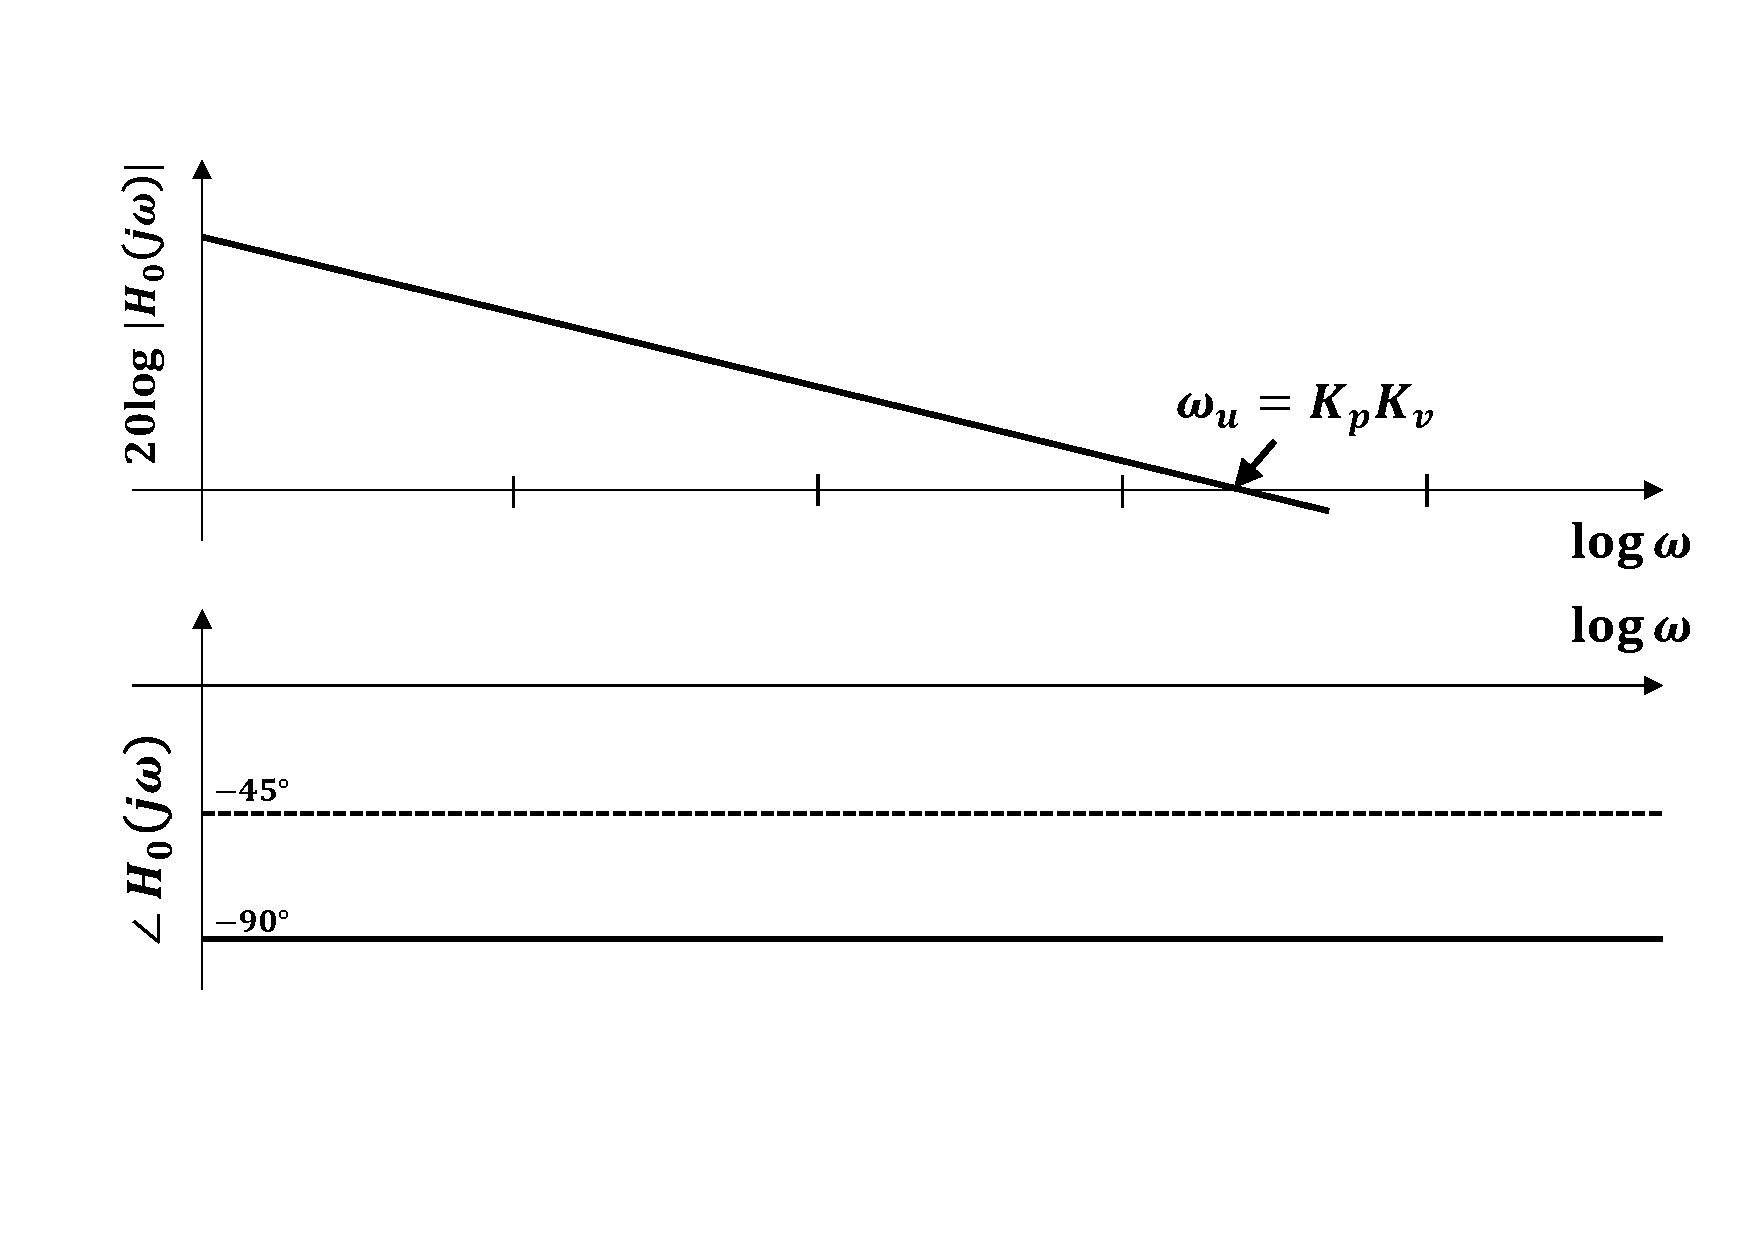
\includegraphics[width=120mm]{figures/pllbode.pdf}
\caption{PLLの伝達関数モデルのボード線図}
\label{pllbode}
\end{center}
\end{figure}
ユニティゲイン角周波数$\omega_u$は$\omega_u=K_pK_v$となる.ここで注目すべきは,PLLは本質的に積分器であることである(伝達関数に$1/s$の項が存在することに注意).これは,VCOが周波数を出力することに対して,PLLの出力は位相であり,位相は周波数の積分として表されるからである.\par
PLLは負帰還回路の一種であるから,安定した動作のためには適切な位相余裕を確保する必要がある.式(3.2)において,位相が回転する要素を含むものはループフィルタの伝達関数$F(s)$と積分要素$1/s$であり,$1/s$は位相が常に$90 ^ \circ$遅れる要素である.したがって,例えば位相余裕を$60 ^ \circ$確保したい場合,$F(s)$で許容される位相遅れは$30 ^ \circ$のみ$(180-90-60=30)$ということになる.よって,LPFの設計が不適当である場合,位相余裕を十分確保できず動作が不安定になるか,最悪の場合正帰還となり異常動作する可能性がある.次項では,以上の内容を踏まえ,具体的なループフィルタのトポロジーについて検討する.

\subsection{ループフィルタの特性比較}
ループフィルタに要求される条件は,前項で述べたとおり適切な位相余裕を確保することと,PFDの出力パルスを十分に平滑化することの2点である.本項では,図\ref{filter}(a)-(c)に示す代表的な3つのループフィルタの諸特性について述べる.

\begin{figure}[t]
\begin{center}

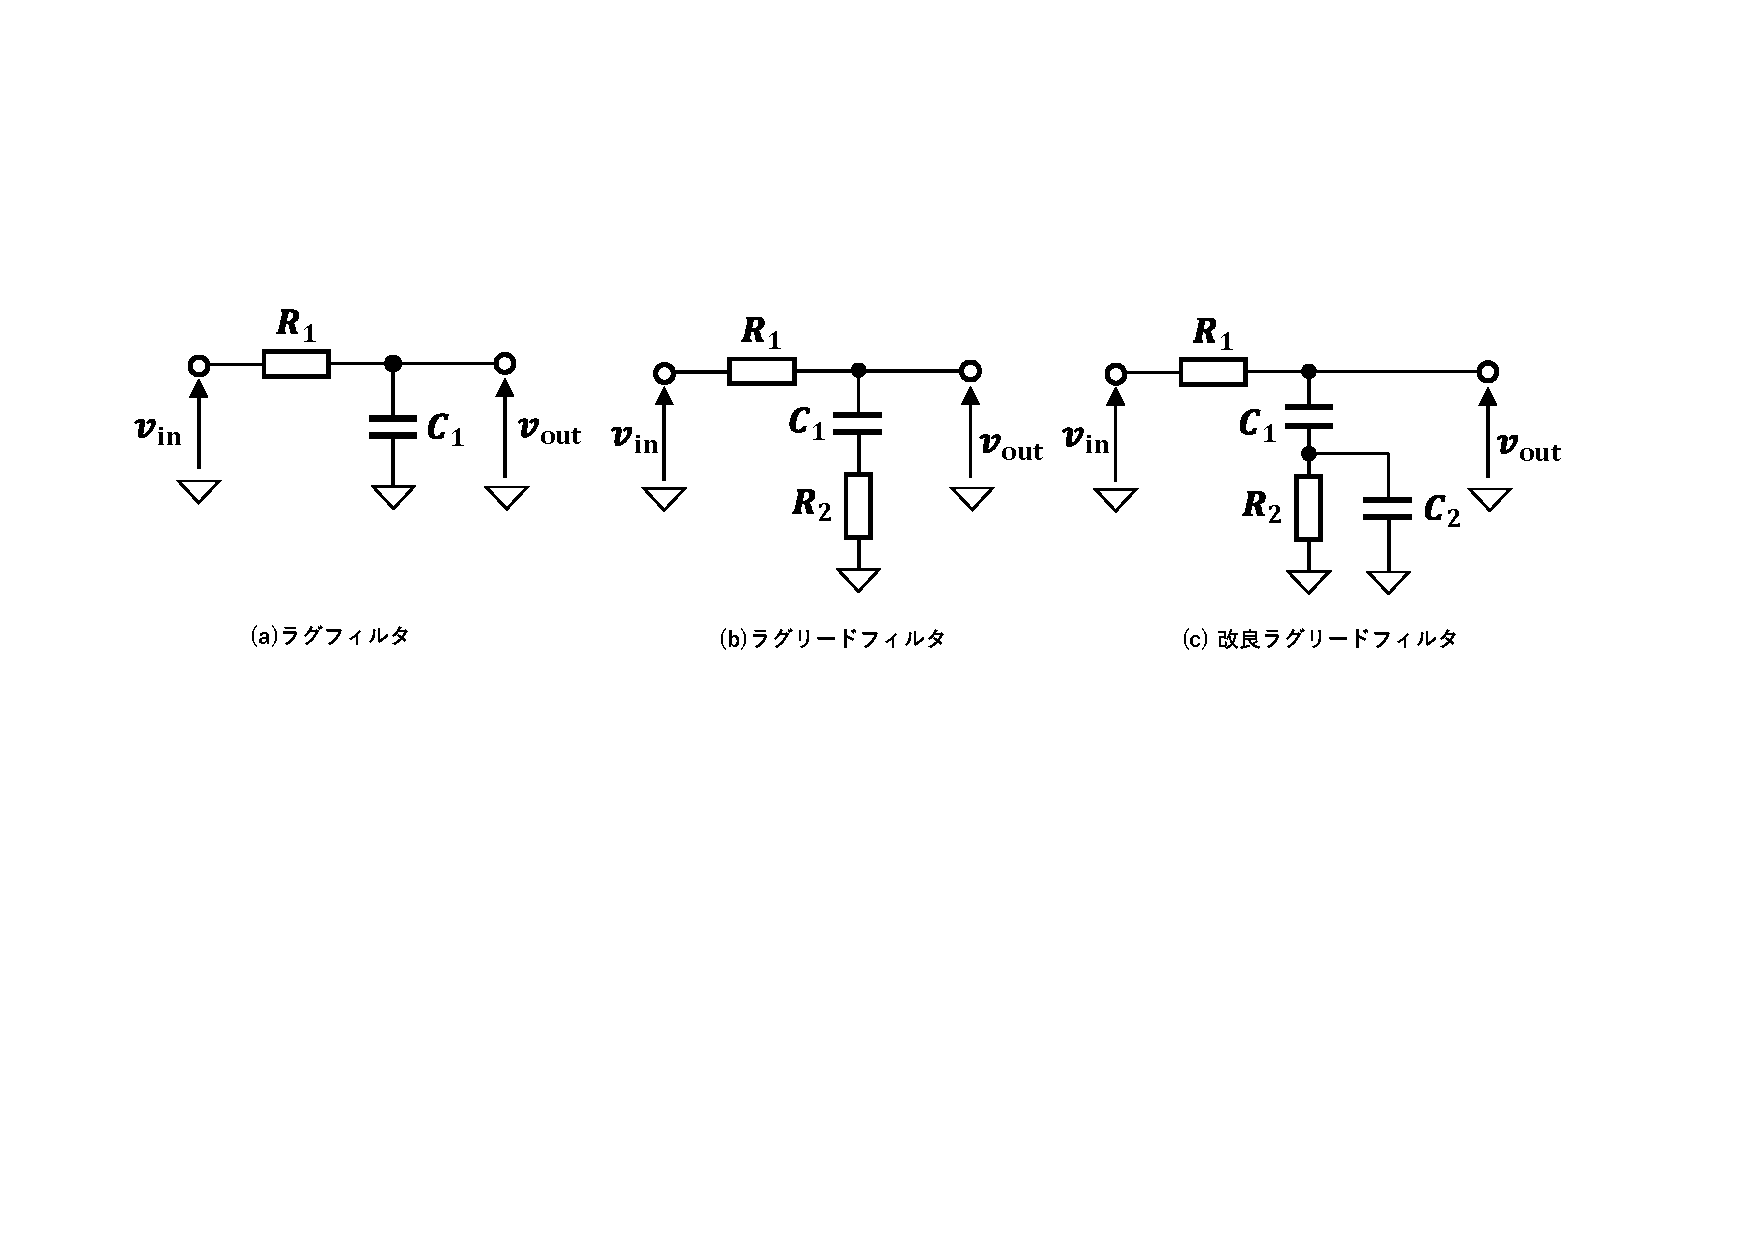
\includegraphics[width=150mm]{figures/filter.pdf}
\caption{ループフィルタ}
\label{filter}

\end{center}
\end{figure}

\subsubsection{ラグフィルタ}
ラグフィルタは,図\ref{filter}(a)に示すように,最も単純な一次の$RC$フィルタであり,その伝達関数$F(s)$は

\begin{align}
F_{lag}(s)=\frac{1}{1+sC_1R_1}
\end{align}
で与えられ,折れ線近似を用いてボード線図を書くと図\ref{lag}のようになる.このフィルタは,同図から明らかなように高周波域で位相遅れが$90 ^ \circ$に漸近するため,十分な位相余裕を確保することができない.仮に,ユニティゲイン角周波数$\omega_u$が同図中のような位置にあった場合,位相余裕はほぼ零に近いことになる.遮断周波数を高くすると,位相余裕は増大するが(ボード線図を右にシフトすると考えれば良い),その分高調波の除去能力は減少する.したがって,この回路は十分な減衰能力と位相余裕を両立させることができず,あまり用いられない\cite{Yanagisawa1998}.

\subsubsection{ラグリードフィルタ}
ラグリードフィルタは,図\ref{filter}(b)に示すようにラグフィルタに抵抗$R_2$を付加したものであり,ループフィルタとして広く用いられているものである.このフィルタの伝達関数$F_{lag-lead}(s)$は
\begin{align}
F_{lag-lead}(s)=\frac{R_2+\cfrac{1}{sC_1}}{R_1+R_2+\cfrac{1}{sC_1}}=\frac{1+sC_1 R_2}{1+sC_1(R_1+R_2)}=\frac{F_1(s)}{F_2(s)}
\end{align}
で与えられる.上式は,一次進み要素$F_1(s)$と一次遅れ要素$F_2(s)$のカスケード接続と考えることができる.したがって$F_{lag-lead}(s)$のボード線図は$F_1(s),F_2(s)$のボード線図の足し合わせで書くことができ,折れ線近似を用いてボード線図を書くと図\ref{lead}のようになる.\par 
ラグリードフィルタの特徴は,高域において位相が戻り,位相遅れが零に漸近することである.これは,高域でキャパシタを短絡とみなせると考えると理解しやすい.この特性により十分な位相余裕を確保することができることから,ループフィルタとして広く用いられている.一方で,高域における減衰は$R_2/(R_1+R_2)$に制限される.高域利得を下げるには,$R_2$を小さくするか$R_1$を大きくすればよいが,前者の場合はラグフィルタに近づくため十分な位相戻りが得られなくなり,後者の場合は遮断角周波数が下がり即応性が悪くなるというトレードオフが存在する.

\subsubsection{改良ラグリードフィルタ}
前項で述べたラグリードフィルタの欠点を改善するために,キャパシタ$C_2$を付加したものが図\ref{filter}(c)の回路である.文献\cite{Enzaka2014}ではこの回路がラグリードフィルタとして紹介されているが,ここでは図\ref{filter}(b)の回路と区別するために改良ラグリードフィルタと呼称する.このフィルタの伝達関数$F_{imp}(s)$は
\newpage
\begin{align}
F_{imp}(s) &= \frac{\cfrac{1}{sC_1}+\cfrac{R_2}{1+sC_2R_2}}{R_1+\cfrac{1}{sC_1}+\cfrac{R_2}{1+sC_2R_2}} \\
&=\frac{\cfrac{1+sC_2R_2+sC_1R_2}{sC_1(1+sC_2R_2)}}{R_1+\cfrac{1+sC_2R_2+sC_1R_2}{sC_1(1+sC_2R_2)}} \\ 
&=\frac{s(C_1R_2+C_2R_2)+1}{s^2 C_1C_2R_1R_2+s\left\{C_1(R_1+R_2)+C_2R_2 \right\}}
\end{align}
で与えられる.上式で与えられるフィルタの中域の利得はおおよそ$R_2/(R_1+R_2)$で与えられ,中域において十分な減衰を得るためには$R_1 \gg R_2$でなければならない.この条件を加味すると,式(3.7)は近似的に
\begin{align}
F_{imp}(s) & \simeq \frac{s(C_1R_2+C_2R_2)+1}{s^2 C_1C_2R_1R_2+s\left\{C_1R_1+C_2R_2 \right\}} \\
&=\frac{s(C_1R_2+C_2R_2)+1}{(s+C_1R_1)(s+C_2R_2)} \\
&=F_3(s)\cdot \frac{1}{F_4(s)} \cdot \frac{1}{F_5(s)}
\end{align}
となり,$F_{imp}(s)$は一次進み要素$F_3(s)$と2つの一次遅れ要素$F_4(s),F_5(s)$のカスケード接続の形で表すことができ,そのボード線図は図\ref{lag-lead}のようになる.改良ラグリードフィルタは,低域で遅れた位相が中域でいったん戻り,高域で再度遅れていくような特性を持つ.また,高域利得は,ラグリードフィルタと異なり$\mathrm{-20 dB/dec.}$で減衰する.したがって,位相余裕と高域における減衰能力を両立できるという利点がある.\par 
なお,本研究で実装した回路においては,各ループフィルタの性能ならびに定数決定に係る設計コストとの相克を考慮し,ラグリードフィルタを採用した.


\begin{figure}[p]
\begin{center}

\vspace{-1cm}

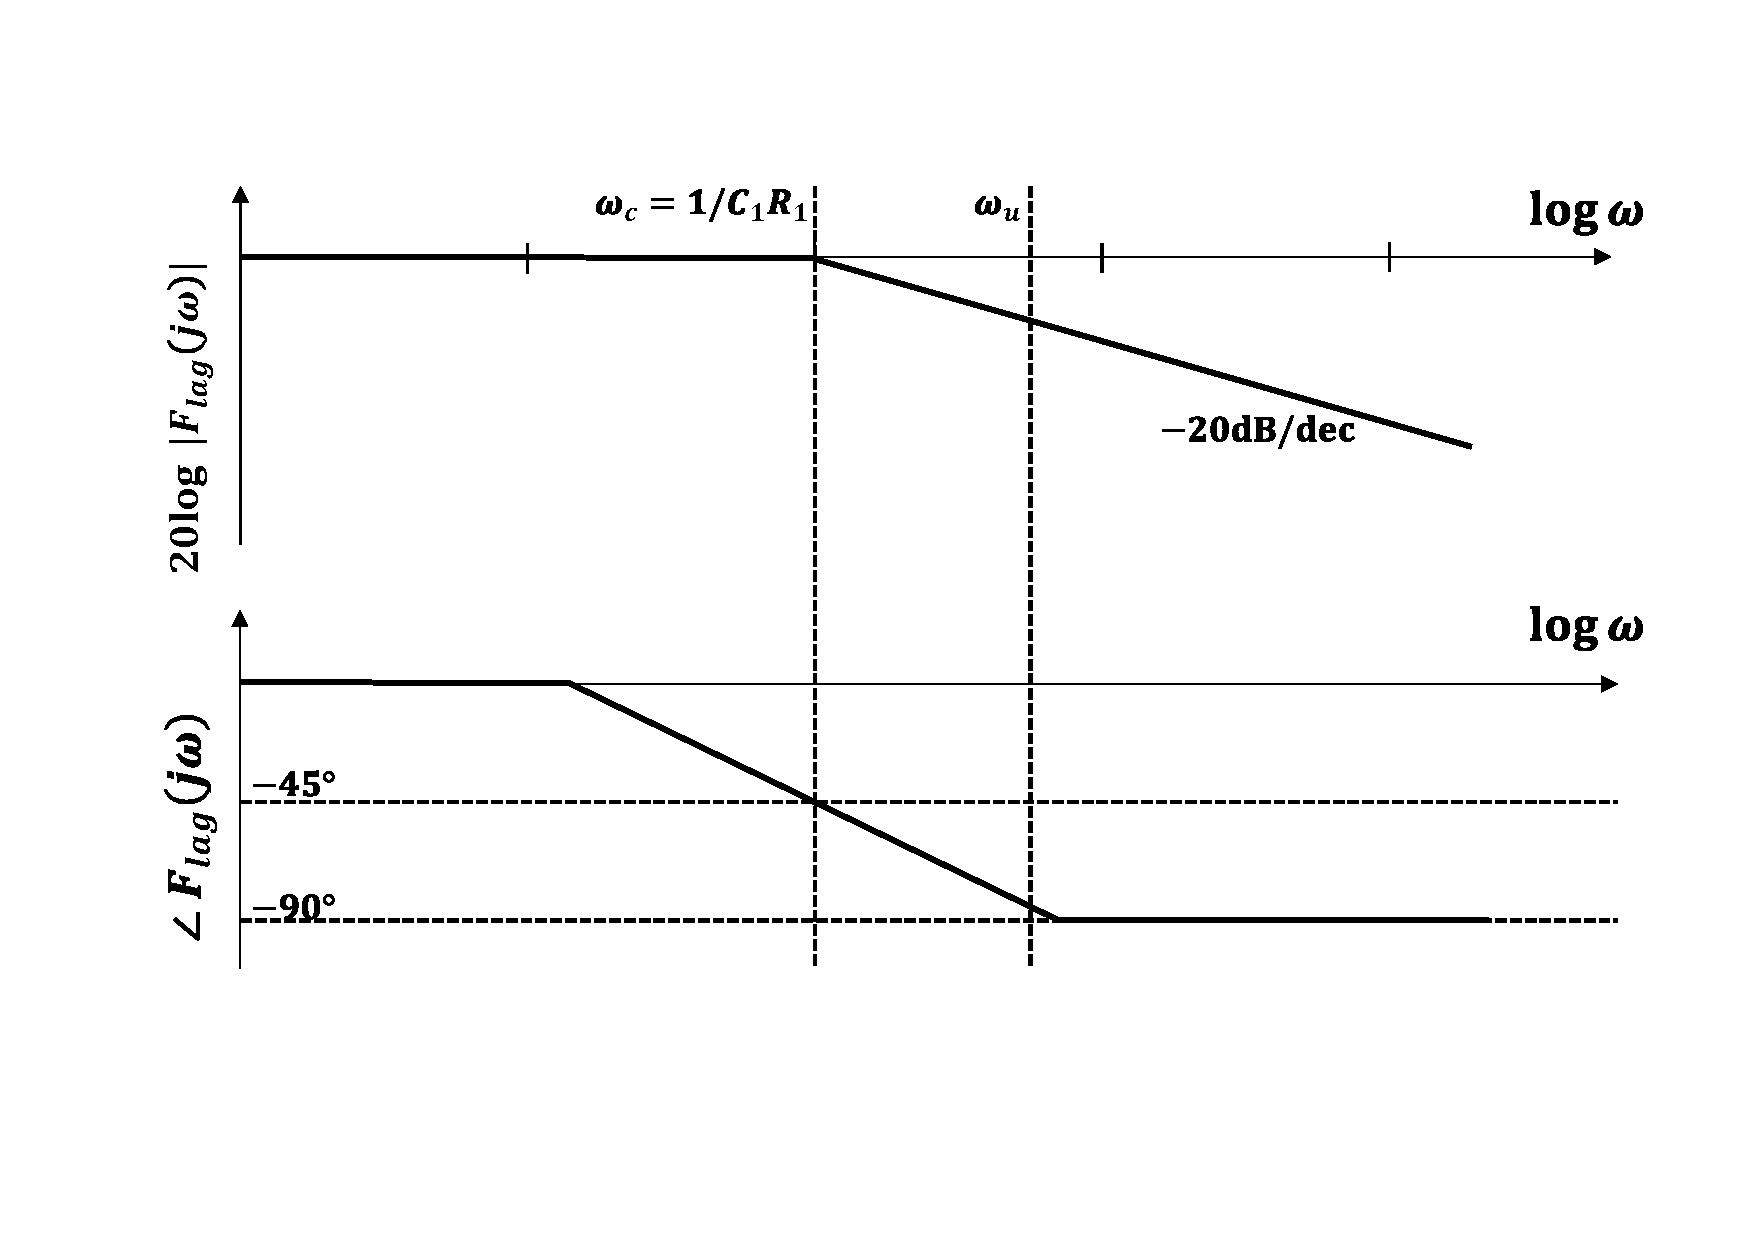
\includegraphics[width=110mm]{figures/lag.pdf}
\caption{ラグフィルタのボード線図}
\label{lag}

\vspace{1cm}

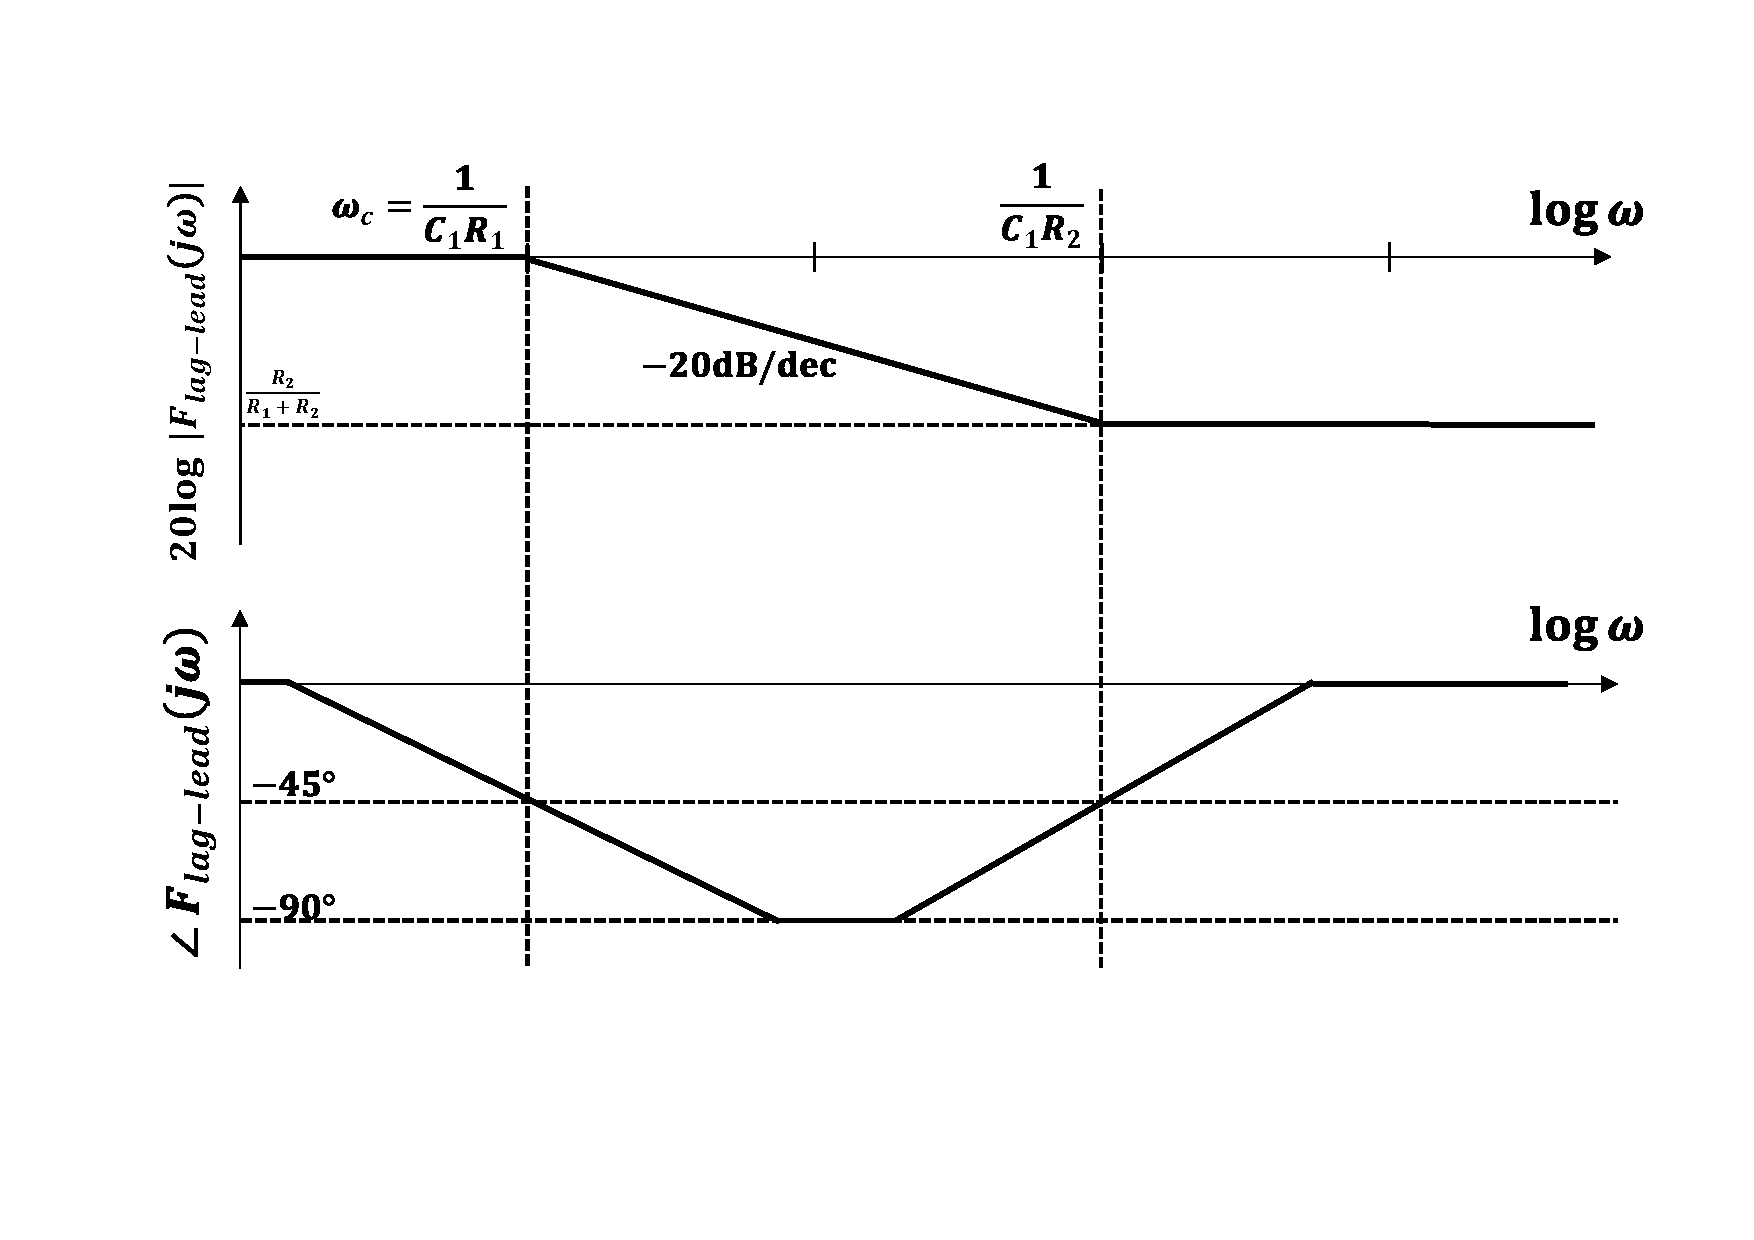
\includegraphics[width=110mm]{figures/lead.pdf}
\caption{ラグリードフィルタのボード線図}
\label{lead}

\vspace{1cm}

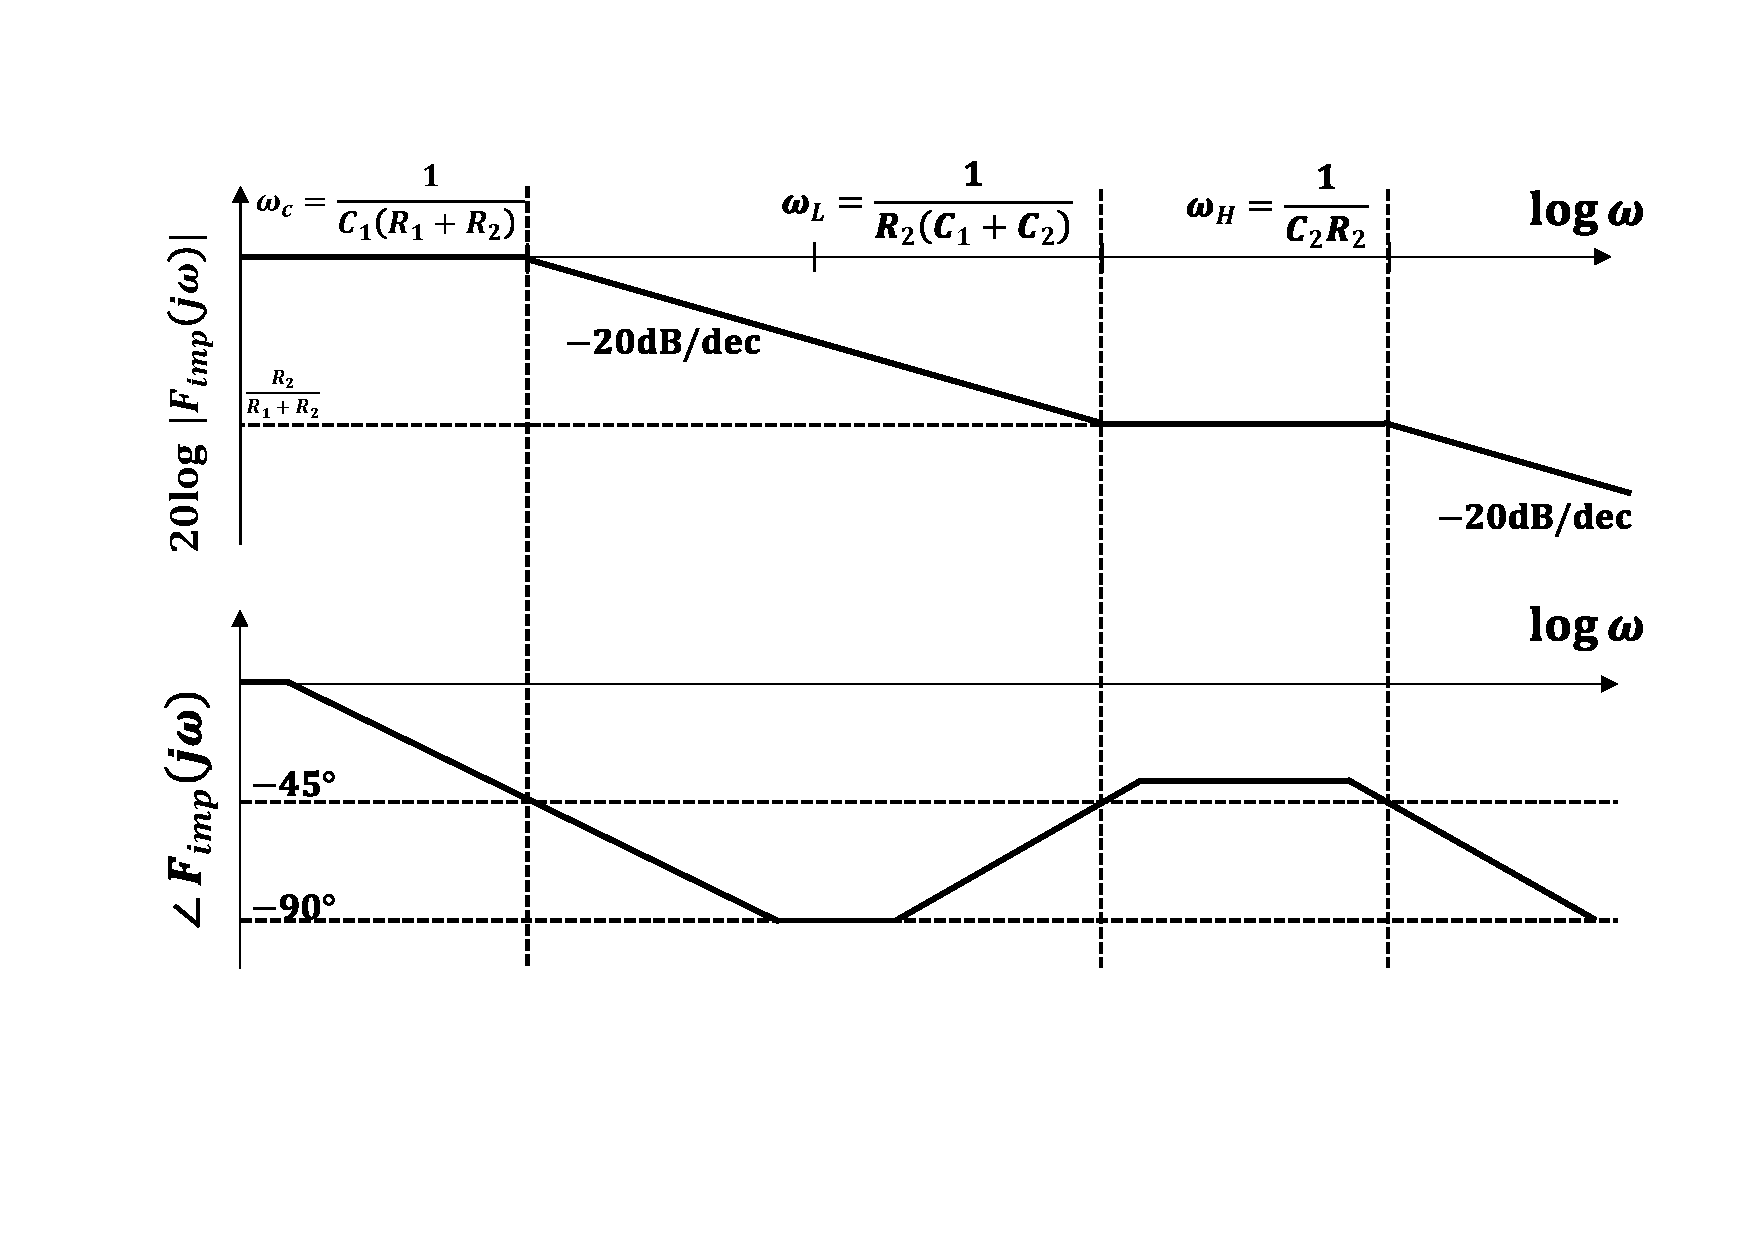
\includegraphics[width=110mm]{figures/lag-lead.pdf}
\caption{改良ラグリードフィルタのボード線図}
\label{lag-lead}

\end{center}
\end{figure}


\subsection{ZRF追従回路の伝達関数モデル}
3.1.1項においては,PLLによりスイッチング電圧$v_{sw}$ならびに電流$i_1$の位相を比較することにより,ZRFの追従動作が実現できることを述べた.本項では,そのような動作を実現するシステムの伝達関数モデルについて述べる.\par 
図\ref{pllblock}に,PLLによるZRF追従回路のブロック図を示す.同図は,図\ref{mr-wpt}における交流電圧源$v_{in}$をVCOに置換し,簡単のため$\rho=r_1=0$として,$i_1$の位相検出用のカレントトランスCTを付加したものある.

\begin{figure}[b]
\begin{center}

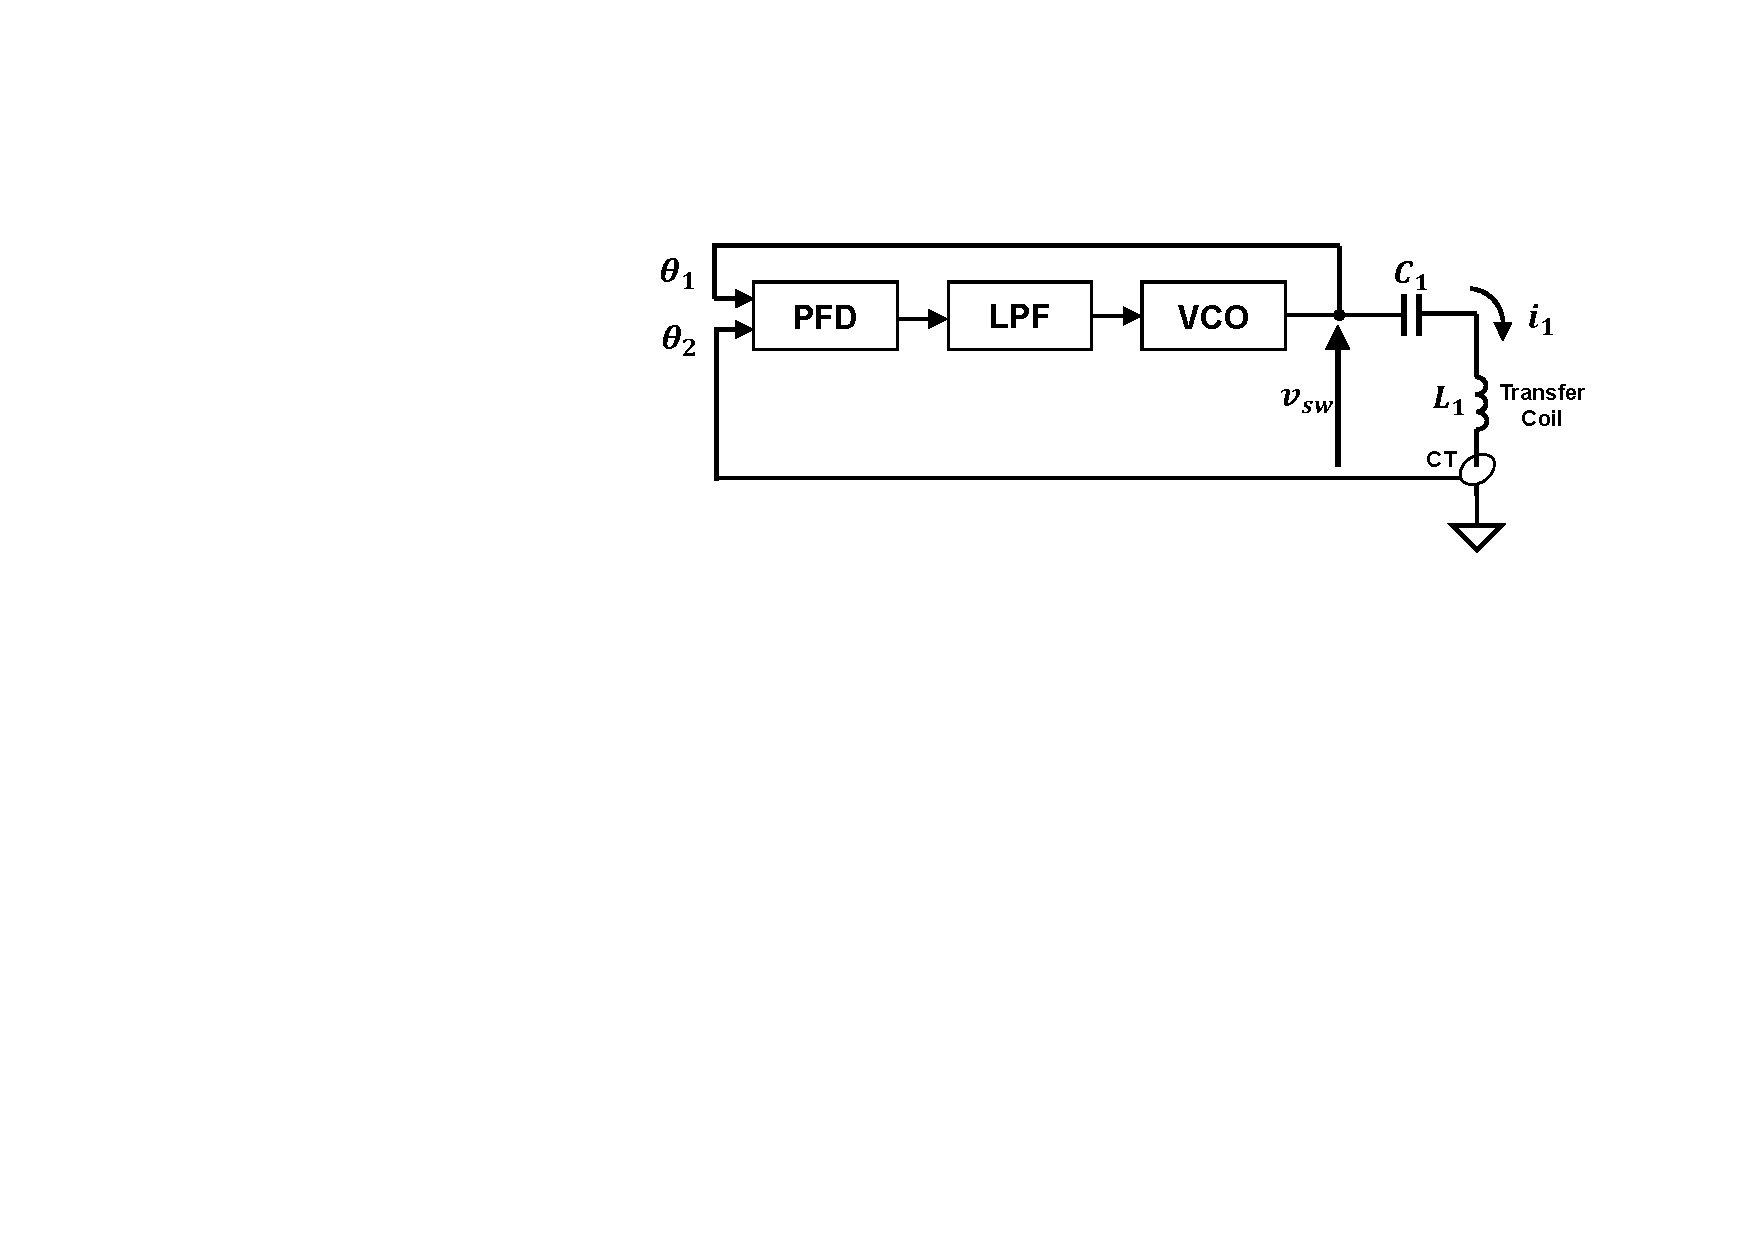
\includegraphics[width=120mm]{figures/pllblock.pdf}
\caption{PLLによるZRF追従回路のブロック図}
\label{pllblock}

\end{center}
\end{figure}

このブロック図を伝達関数モデルとして表現することを考える.PFDとVCOについては,図\ref{pll}と同じように比例要素として扱えばよく,VCOの比例ゲイン$K_v$の次元を$\mathrm{[rad/s/V]}$とすると,その出力は角周波数$\omega_0 \, \mathrm{[rad/s]}$として表せる.ここで取り扱いが難しいのが,$\omega_0$に対する$C_1$と$L_1$による位相回転である.図\ref{argi1}は,ある設計例におけるVCOの出力周波数と$i_1$の位相$\theta_2$の数値計算結果であるが,同図から明らかなように両者は非線形の関係にある.したがって,VCOの出力を(角)周波数として考えた場合,伝達関数を用いてモデリングすることができない.\par
非線形制御系の解析は非常に難しいため,ここでは線形モデルとして扱うことを考える.すなわち,図\ref{pllblock}の回路において,PLLは$f_{ZRF1}$または$f_{ZRF2}$にロックするように動作させることを考慮して,それらの周波数における位相特性曲線の接線を引くことにより,位相特性を線形近似する.図\ref{argi1}における一点鎖線は,例として$f_{ZRF1}$における接線を示したものである.接線の傾きを$K_\theta$とすれば,$\omega_0$に対する位相$\theta_2$は,

\begin{align}
\theta_2 = K_\theta \omega_0
\end{align}

と書ける.以上の内容を考慮すると,図\ref{pllblock}の伝達関数モデルは図\ref{pllmodel}のようになる.なお,$K_\theta$の値は解析的に求めることもできるが,計算が非常に複雑になるため,グラフから図的に求めるのが現実的であると考えられる.

\begin{figure}[h]
\begin{center}

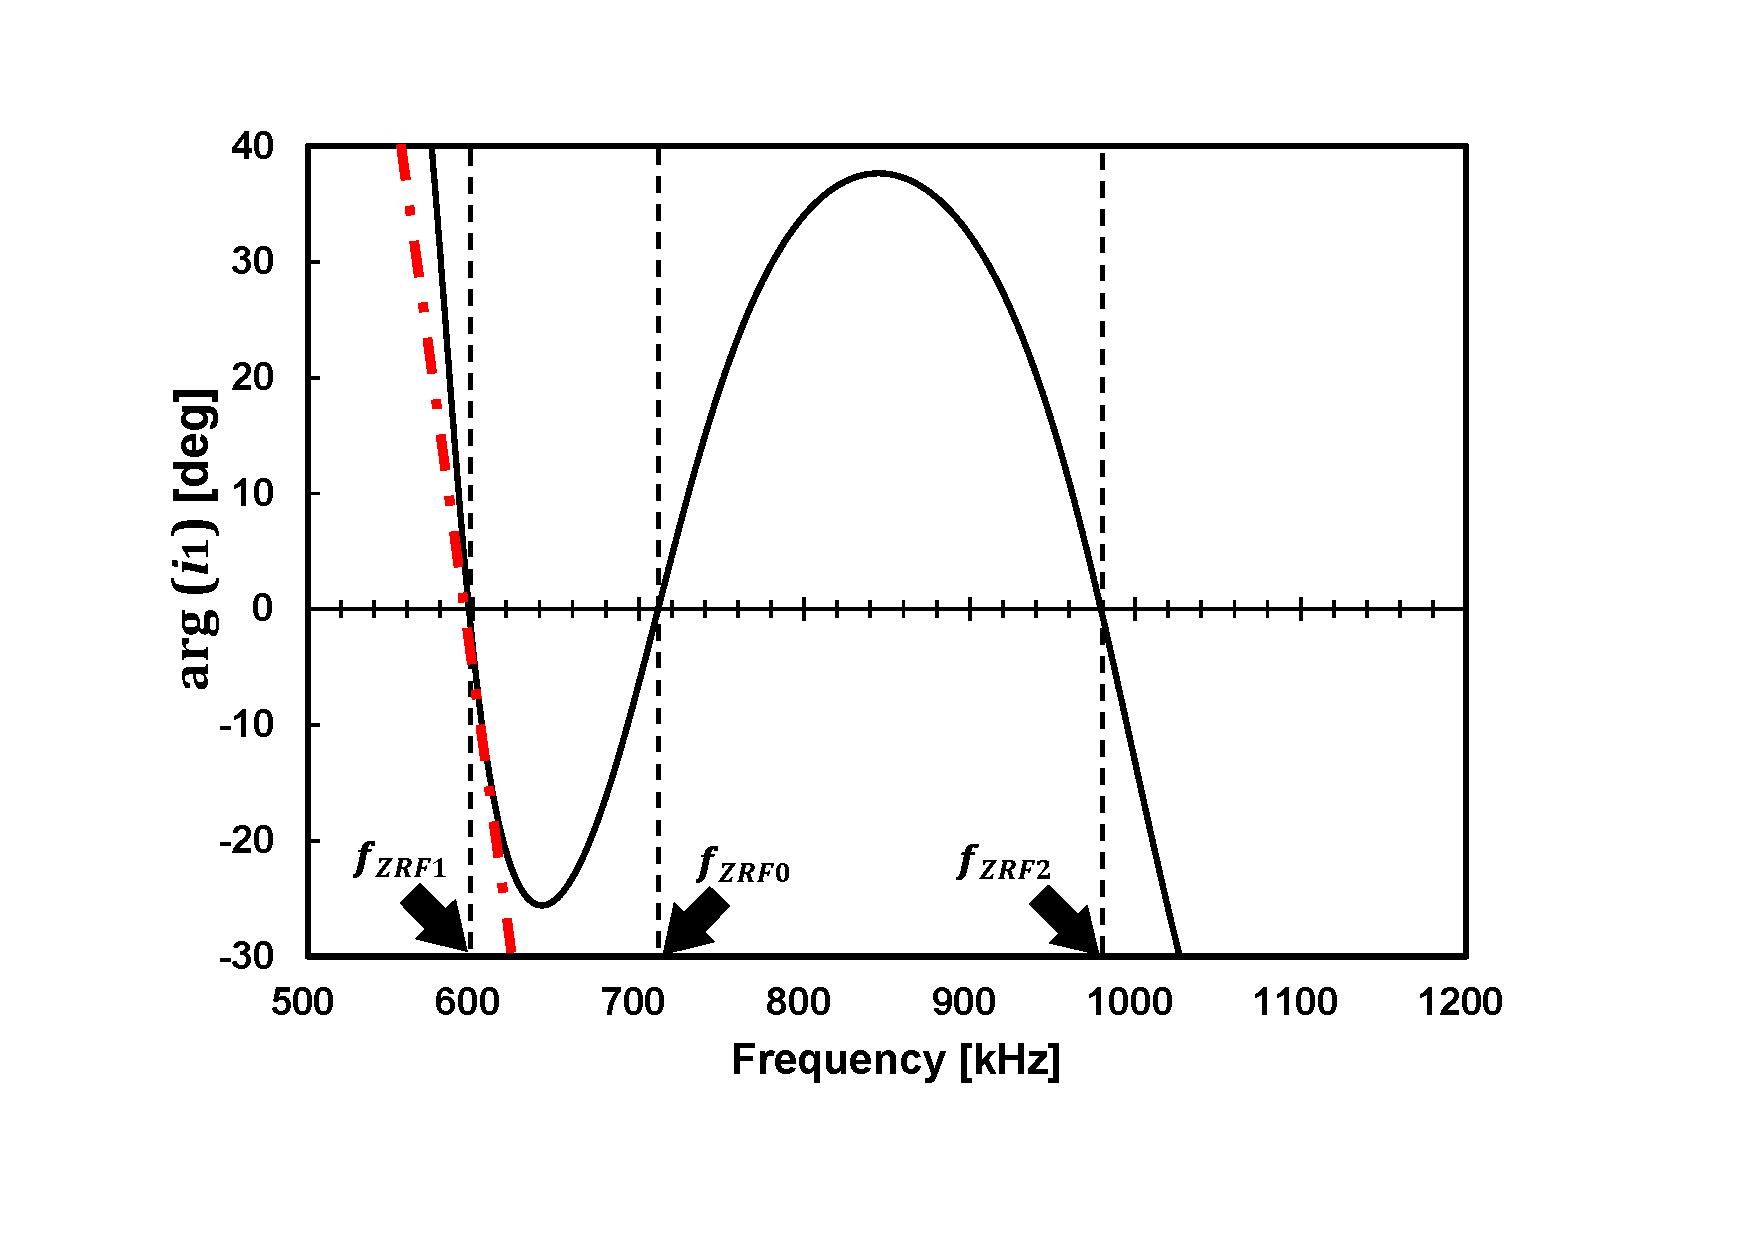
\includegraphics[width=120mm]{figures/argi1.pdf}
\caption{電流$i_1$の位相特性}
\label{argi1}

\vspace{5mm}

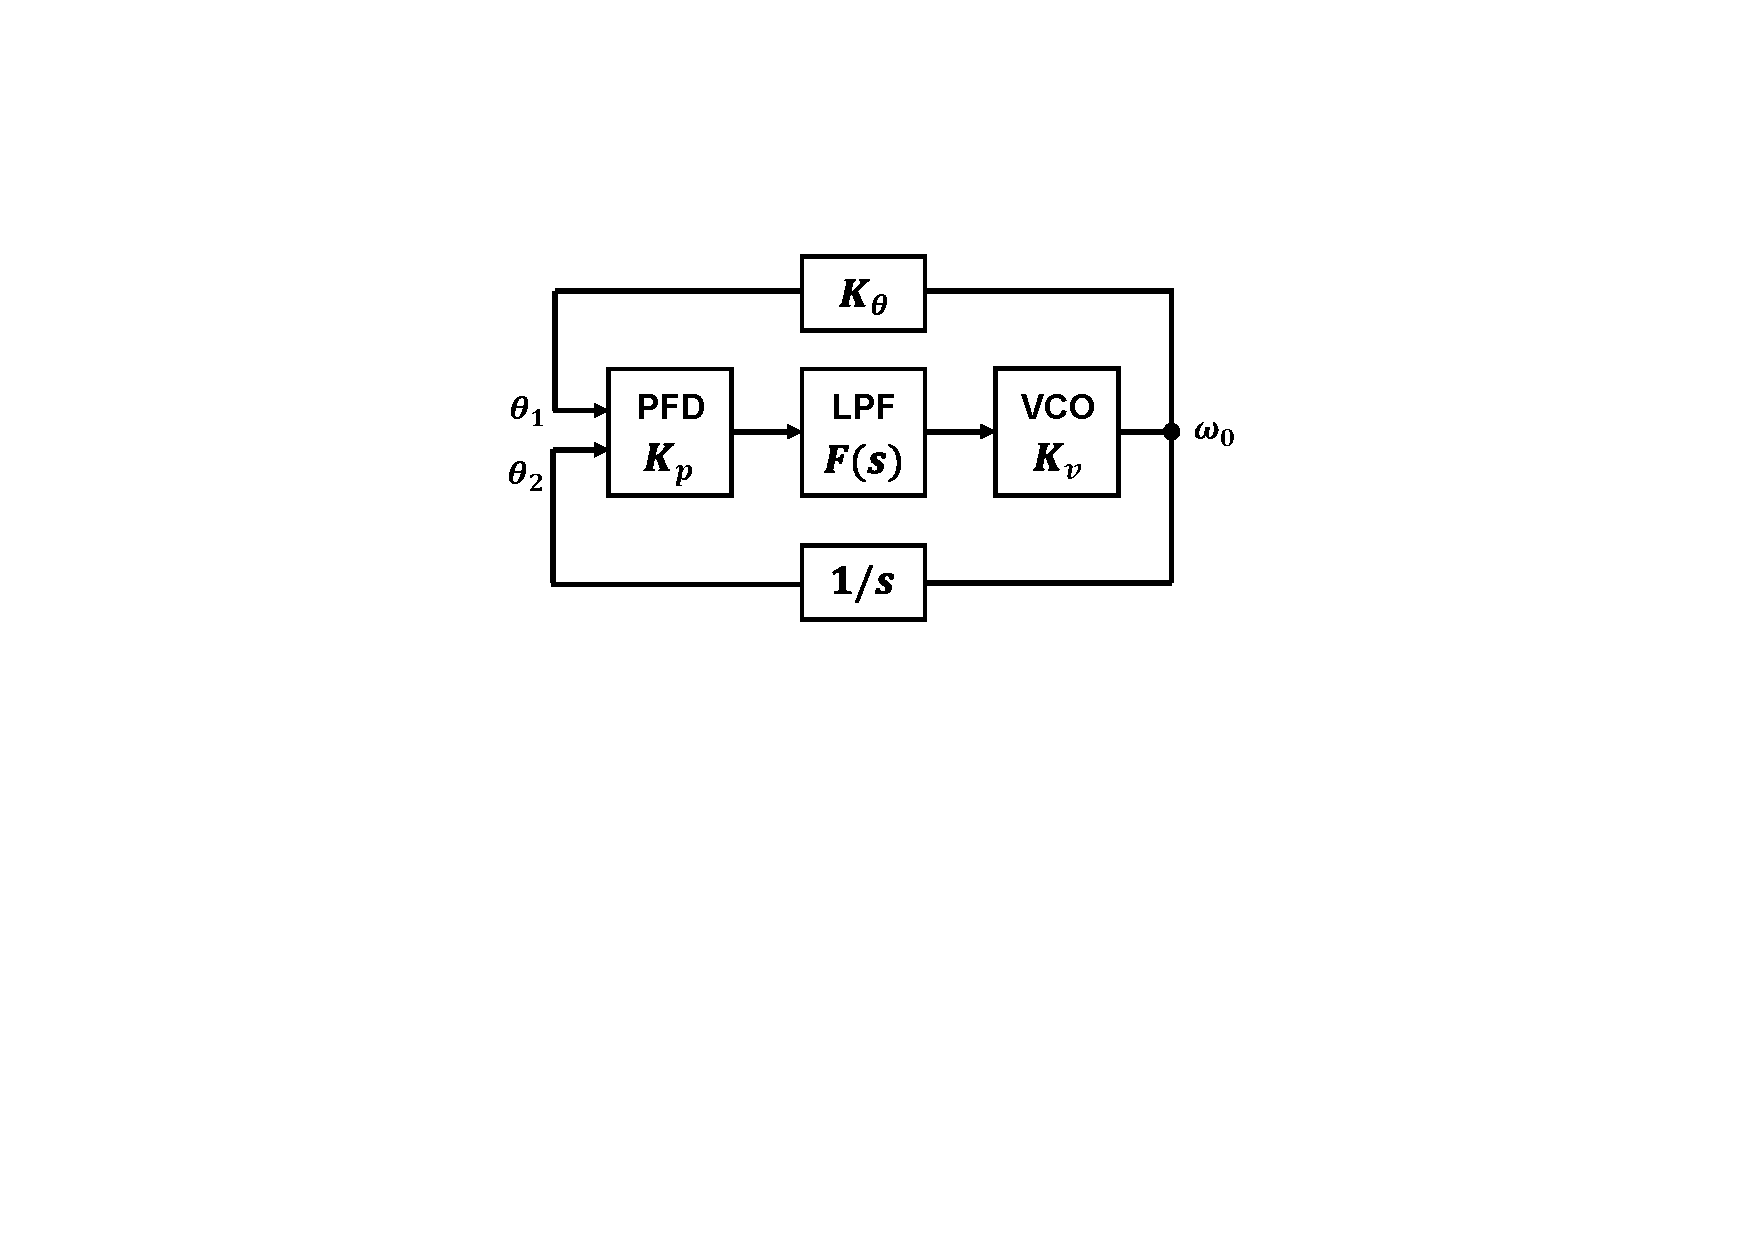
\includegraphics[width=80mm]{figures/pllmodel.pdf}
\caption{ZRF追従回路の伝達関数モデル}
\label{pllmodel}

\end{center}
\end{figure}

\subsection{PLLが所望のZRFでロックすることの証明}
2.1節において図\ref{freqchar}を示して述べたとおり,ZRFは3つ存在し,うち周波数軸上の右端と左端にあるZRFである$f_{ZRF1}, f_{ZRF2}$においては大きな電力を伝送できる.一方,もう一つのZRFである$f_{ZRF0}$においては,出力電力はほぼ極小値となり,大きな電力を伝送することができない.本項では,PLLによるZRFの追従回路が$f_{ZRF1}, f_{ZRF2}$のみでロックし,$f_{ZRF0}$ではロックしないことを,前項で示した伝達関数モデルならびにフルビッツの安定法により示す.\par 
図\ref{pllmodel2}は,図\ref{pllblock}の伝達関数モデルにおいて,VCOの位相雑音として$\omega_d$が重畳されることを想定したモデルである.ただし,$K_p,K_v$はそれぞれPFDとVCOの伝達利得,$K_\theta$は位相特性曲線を線形近似したときの傾きである.$\omega_d$が出力角周波数$\omega_0$に与える影響を調べるため,閉ループ伝達関数$G(s)=\omega_0/\omega_d$を求める.図\ref{pllmodel2}において,
\begin{figure}[b]
\begin{center}

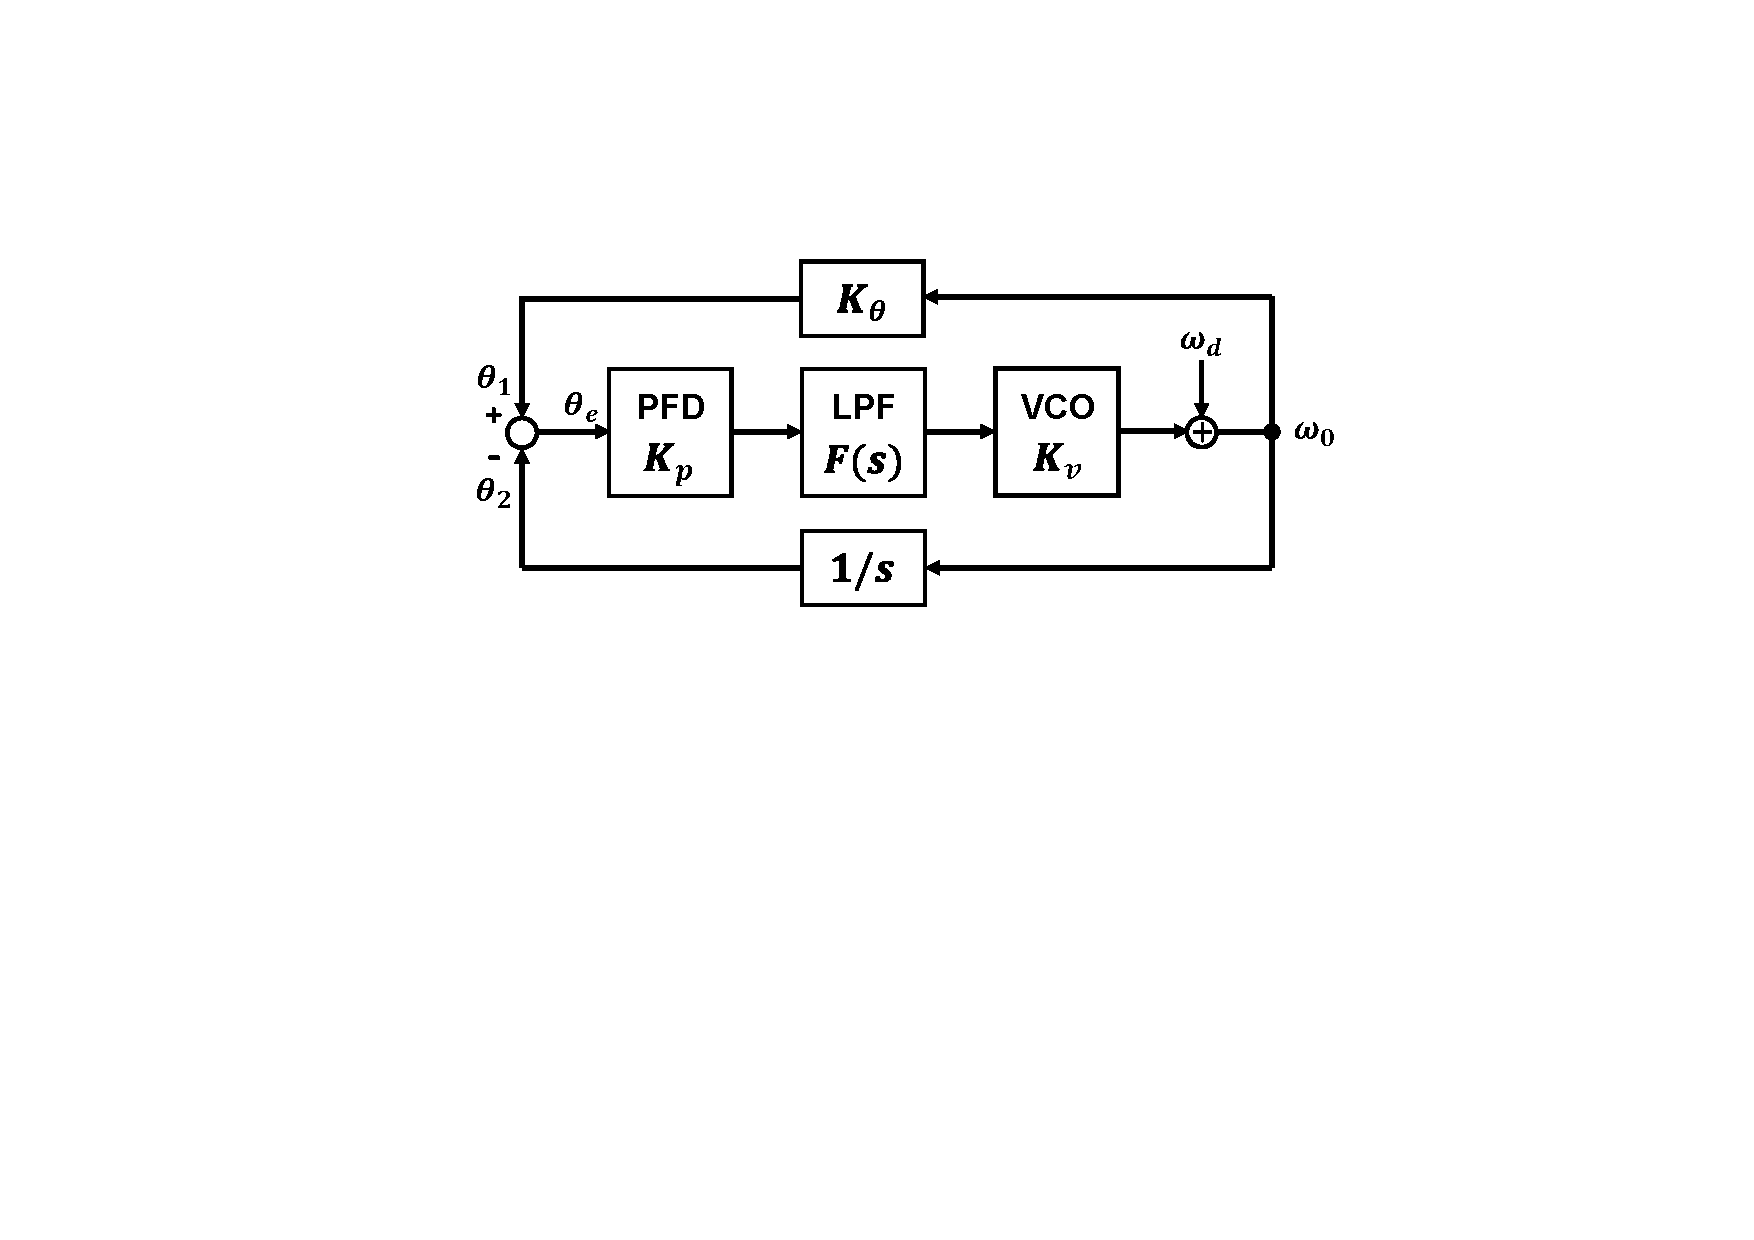
\includegraphics[width=80mm]{figures/pllmodel2.pdf}
\caption{位相雑音$\omega_d$を考慮したZRF追従回路の伝達関数モデル}
\label{pllmodel2}

\end{center}
\end{figure}
\begin{align}
\theta_e=\theta_1-\theta_2=\omega_0 \left(K_\theta-\frac{1}{s} \right) 
\end{align}
\begin{align}
\omega_0=\theta_e K_p K_v F(s)+ \omega_d
\end{align}
が成り立つ.式(3.12)を式(3.13)に代入すれば,
\begin{align}
\omega_0=\omega_0 \left(K_\theta-\frac{1}{s} \right) \cdot K_p K_v F(s)+\omega_d
\end{align}
となる.したがって,
\begin{align}
G(s) \equiv \frac{\omega_0}{\omega_d} &=\cfrac{1}{1-K_p K_v F(s) \left(K_\theta-\frac{1}{s}\right)} \\ 
% &=\cfrac{1}{1-\cfrac{K_pK_vF(s)}{s}(sK_\theta-1)}\\
% &=\frac{s}{s-K_p K_v F(s)(sK_\theta-1)}\\
&=\frac{s}{s(1-K_pK_vK_\theta F(s))+K_pK_vF(s)}
\end{align}
であり,特性方程式は
\begin{align}
s(1-K_pK_vK_\theta F(s))+K_pK_vF(s)=0
\end{align}
となる.以下,図\ref{filter}(a),(b)に示したふたつのループフィルタを用いた場合において,ループが安定となる$K_\theta$の条件をフルビッツの安定判別法により求める.

\subsubsection{ラグフィルタ}
図\ref{filter}(a)に示したラグフィルタの伝達関数$F_{lag}(s)$は,$R_1C_1=\tau$とすれば
\begin{align}
F_1(s)=\frac{1}{1+\tau s}
\end{align}
である.このときの特性方程式は,式(3.17)の$F(s)$に上式を代入して
\begin{align}
s \left(1-K_pK_vK_\theta \cdot \frac{1}{1+\tau s} \right) + \frac{K_pK_v}{1+\tau s}=0
\end{align}
となる.両辺に$1+\tau s$を乗じて整理すると,
\begin{align}
s(1+\tau s) \left(1-K_pK_vK_\theta \cdot \frac{1}{1+\tau s} \right)+K_pK_v =0 \\
s(1+\tau s -K_pK_vK_\theta)+K_pK_v=0 \\
s^2 \tau +s(1-K_pK_vK_\theta)+K_pK_v=0
\end{align}
となり,フルビッツ行列$H_1$は
\begin{align}
H_1=
\begin{pmatrix}
1-K_pK_vK_\theta & 0 \\
\tau & K_pK_v
\end{pmatrix}
\end{align}
と表せる.ループが漸近安定となる条件は,式(3.23)より,
\begin{align}
1-K_pK_vK_\theta>0 
\end{align}
\begin{align}
\begin{vmatrix}
1-K_pK_vK_\theta & 0 \\
\tau & K_pK_v
\end{vmatrix}
=K_pK_v(1-K_pK_vK_\theta)>0
\end{align}
の2つが同時に成立することであるが,$K_pK_v$が常に正であることは考慮すれば,この2条件は
\begin{align}
1-K_pK_vK_\theta>0
\end{align}
のみとなり,これを$K_\theta$について解くと
\begin{align}
K_\theta<\frac{1}{K_pK_v}
\end{align}
となる.さらに,$K_pK_v \gg 1$と仮定すれば,
\begin{align}
K_\theta<0
\end{align}
と表せる.したがって,$K_\theta$が正のときは出力$\omega_0$は発散し,図\ref{argi1}より$f_{ZRF0}$のときの位相特性曲線の傾き$K_\theta$は正であるから,PLLは$f_{ZRF0}$にロックしない.

\subsubsection{ラグリードフィルタ}
図\ref{filter}(b)に示したラグフィルタの伝達関数$F_{lag-lead}(s)$は,$C_1(R_1+R_2)=\tau_1, \, C_1R_1=\tau_2$とすれば
\begin{align}
F_2(s)=\frac{1+\tau_2 s}{1+\tau_1 s}
\end{align}
である.このときの特性方程式は,式(3.17)の$F(s)$に上式を代入して
\begin{align}
s \left(1-K_pK_vK_\theta \cdot \frac{1+\tau_2 s}{1+\tau_1 s} \right) + K_pK_v \cdot \frac{1+\tau_2 s}{1+\tau_1 s}=0
\end{align}
となる.両辺に$1+\tau_1 s$を乗じて整理すると,
\begin{align*}
s(1+\tau_1 s)\left(1-K_pK_vK_\theta \cdot \frac{1+\tau_2 s}{1+\tau_1 s} \right)+K_pK_v(1+\tau_2 s)=0 \\ 
% s(1+\tau_1s-(1+\tau_2s)K_pK_vK_\theta)+K_pK_v(1+\tau_2 s)=0\\
% s+s^2\tau_1-sK_pK_vK_\theta(1+\tau_2s)+K_pK_v(1+\tau_2s)=0 \\
s^2(\tau_1-K_pK_vK_\theta \tau_2)+s(1-K_pK_vK_\theta+K_pK_v\tau_2)+K_pK_v=0
\end{align*}

となり,フルビッツ行列$H_2(s)$は
\begin{align}
H_2=
\begin{pmatrix}
1-K_pK_vK_\theta+K_pK_v\tau_2 & 0 \\
\tau_1-K_pK_vK_\theta \tau_2 & K_pK_v
\end{pmatrix}
\end{align}
と書ける.漸近安定条件は,ラグフィルタのときと同様に考えれば
\begin{align}
1-K_pK_vK_\theta+K_pK_v\tau_2>0
\end{align}
となり,これを$K_\theta$について解けば
\begin{align}
K_\theta<\frac{1}{K_pK_v}-\tau_2 \simeq -\tau_2
\end{align}
となり,以上より,ラグフィルタのときと同様に,$K_\theta$が正のときはPLLがロックしないことが示せた.

\section{回路構成ならびにシミュレーション}
\subsection{全体構成}
図\ref{entireblock}に,ここまでに述べた原理に基づいて設計した,PLLによるZRF追従回路の全体図を示す.$C_1$と$L_1$で構成されたMR-WPT回路を,2つのnチャネルMOSFETからなるハーフブリッジで駆動している.2つのFETは,VCOの出力信号とその反転信号により交互に導通し,振幅が$V_{SW}$の矩形波$v_{sw}$を生成する.各FETのスイッチング信号には,デッドタイム生成回路(Dead time Generator)によりデッドタイムを付加している.カレントトランスCTによって検出される電流$i_1$は,電流-電圧変換・波形整形回路(Current to Voltage Converter and Waveform Shaping)により正弦波状の電流から矩形波の電圧信号に変換された後,電圧$v_{sw}$とともに遅延補正回路(Delay Compensator)を通過し,PFDに入力される.電流-電圧変換・波形整形回路においては,適当な抵抗で電流-電圧変換を行った後,コンパレータを用いて矩形波信号を得ている.デッドタイム生成回路ならびに波形整形・遅延補正回路については,次項において詳しく述べる.
\begin{figure}[h]
\begin{center}

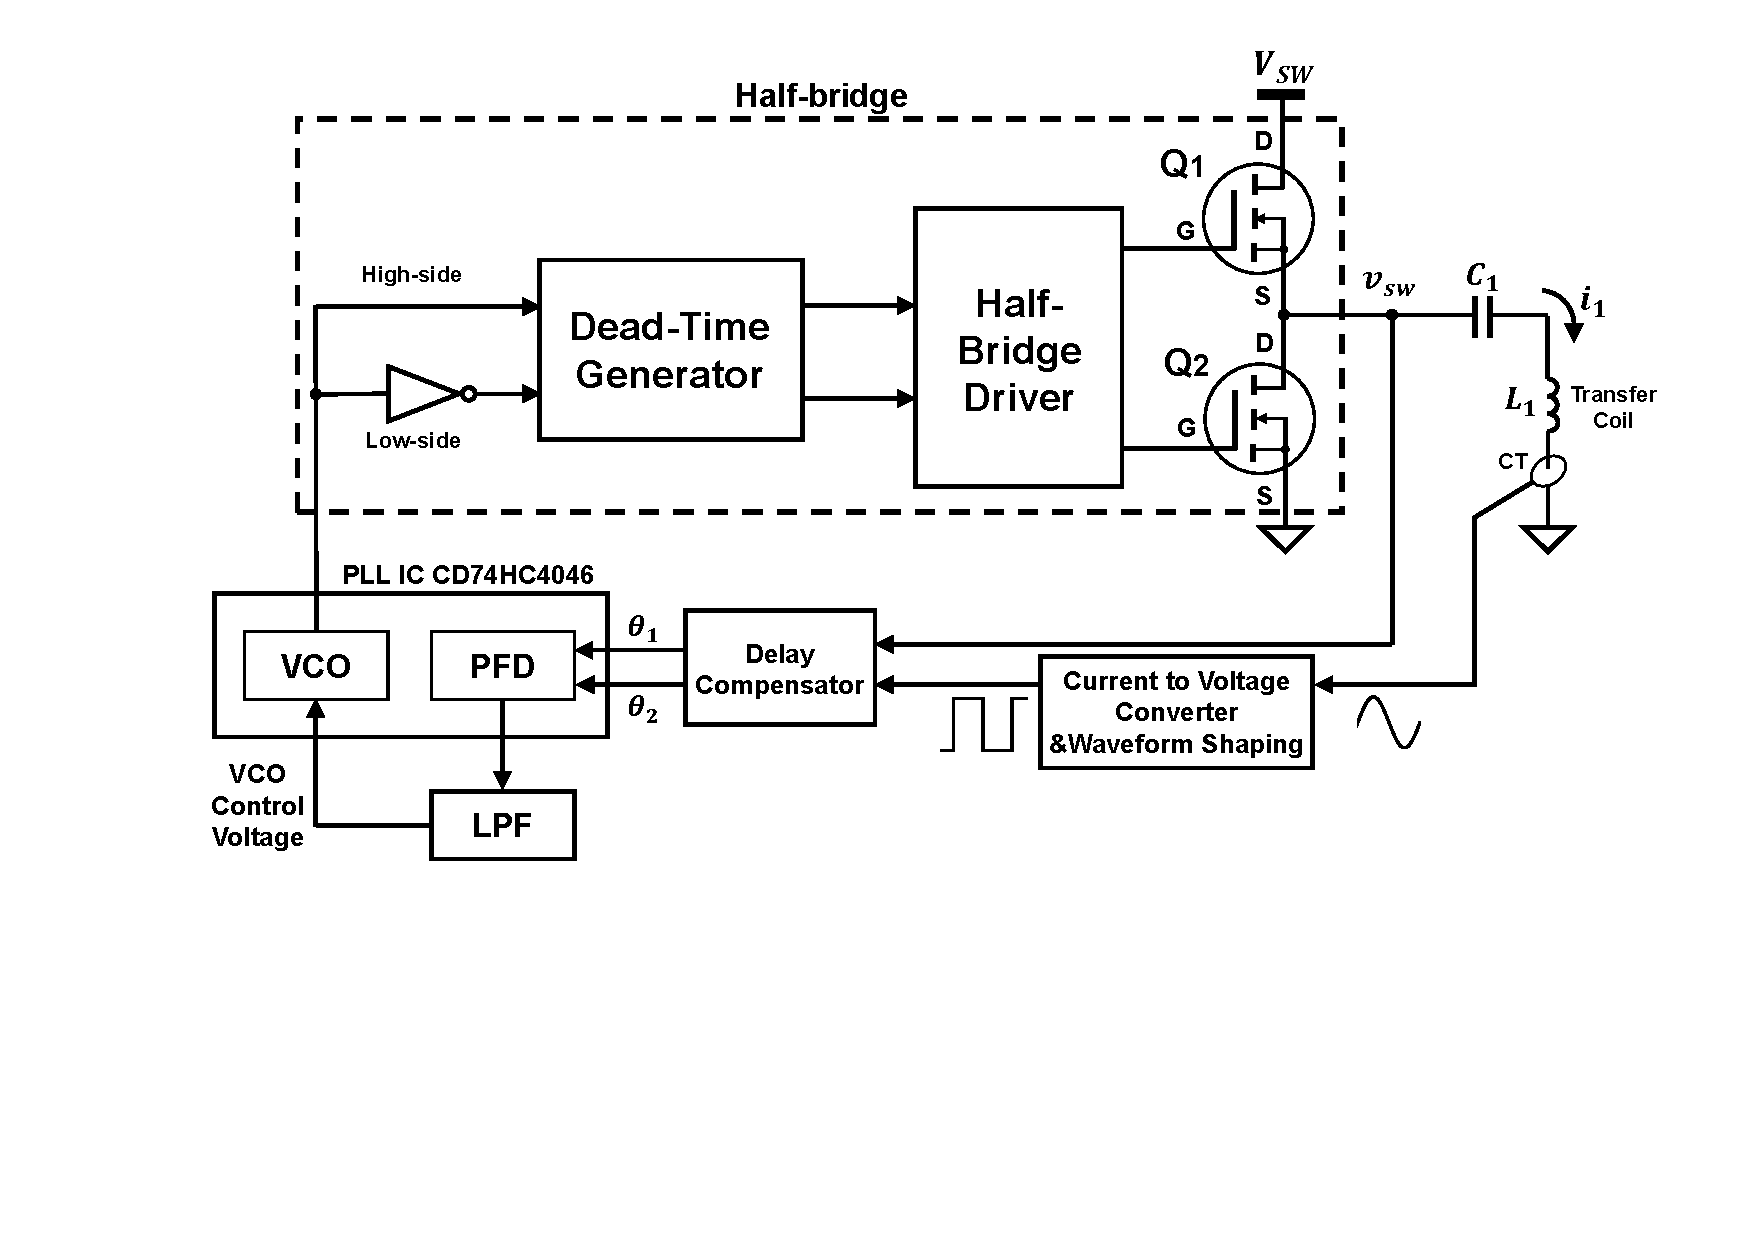
\includegraphics[width=130mm]{figures/entireblock.pdf}
\caption{PLLによるZRF追従回路の全体構成図}
\label{entireblock}

\end{center}
\end{figure}

\subsection{内部回路}
\subsubsection{デッドタイム生成回路}
図\ref{deadtimegenerator}に示すデッドタイム生成回路は,ハーフブリッジ回路における2つのFETの同時導通に起因する短絡を防ぐため,両FETがターンオフするデッドタイム$t_{dead}$を挿入する回路である.例として同図回路の上段について説明する.VCOの出力信号(Duty比50\%の矩形波)は,バッファを通過しダイオード$D_1$,抵抗$R_1$ならびにキャパシタ$C_1$から成る回路に印加される.バッファの出力信号が立ち上がるときは,$D_1$は開放状態とみなすことができ,コンパレータ1の入力信号は$R_1$と$C_1$で決定される適当な時定数で遅延する.一方,バッファの出力信号が立ち下がるときは,$D_1$を短絡とみなすことができ,コンパレータ1の入力信号は遅延しない.この結果,コンパレータ1の出力信号は,VCOからの出力信号に対して立ち上がりが一定時間遅延する矩形波信号となる.遅延時間は,キャパシタ$C_1$ならびにコンパレータ1の反転入力端子に接続されている可変電圧源$V_{REF1}$の値を可変することにより調整する.\par
以上の動作を,図\ref{deadtimegenerator}下段の回路において,VCO出力の反転信号に対しても行う.これにより,各コンパレータの出力信号,すなわちハイサイドFETとローサイドFETの駆動信号が両方ともLOWレベルになる時間$t_{dead}$が生成され,FETの同時導通を防ぐことができる.

\begin{figure}[h]
\begin{center}

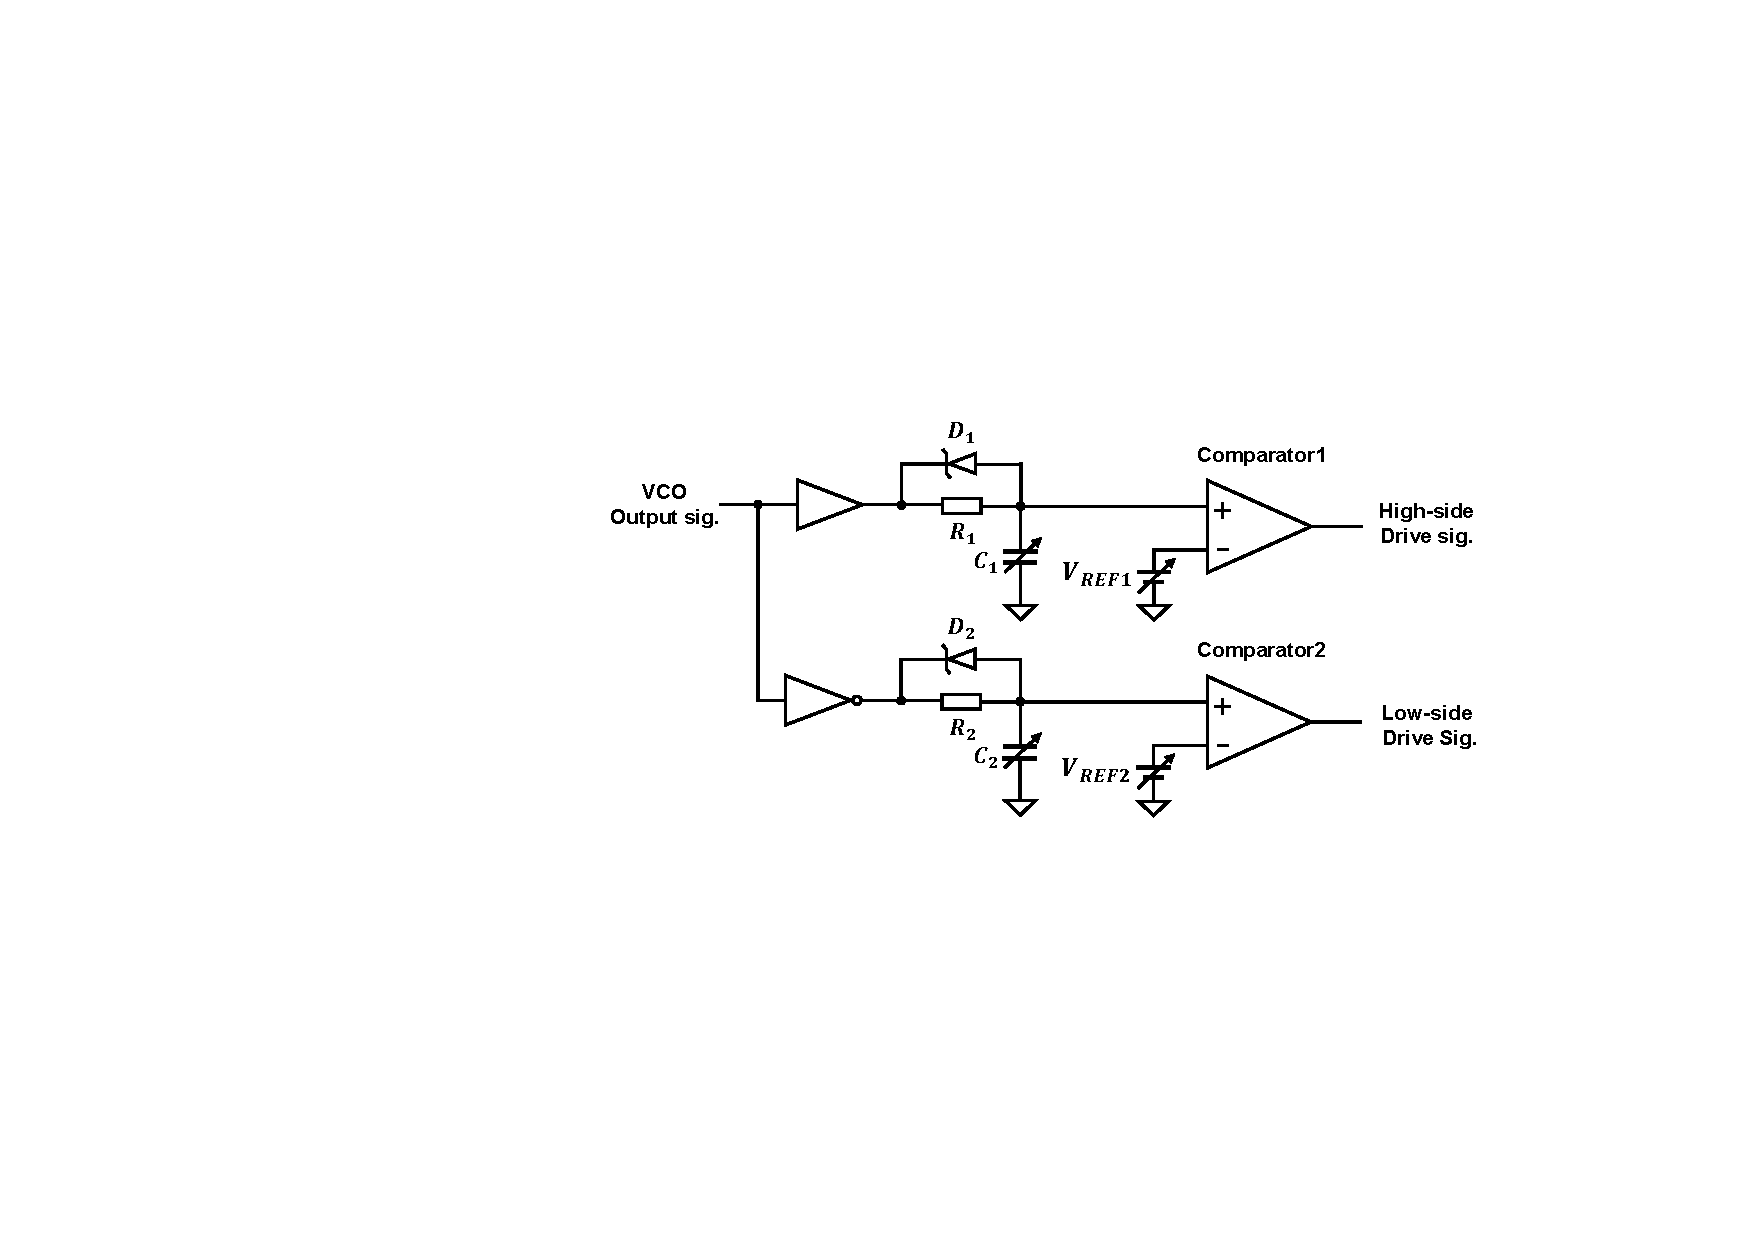
\includegraphics[width=120mm]{figures/deadtimegenerator.pdf}
\caption{デッドタイム生成回路}
\label{deadtimegenerator}

\end{center}
\end{figure}

\subsubsection{波形整形・遅延補正回路}
波形整形・遅延補正回路は,カレントトランスCTで検出されるスイッチング電流$i_1$を電圧に変換し矩形波に変換するとともに,コンパレータならびにアイソレータの伝搬遅延による影響を補正する回路である.図\ref{delaycompensator}は,電流$i_1$ならびに電圧$v_{sw}$の位相が等しい状態を図示している.$i_1$は,抵抗$R_1$により適当な大きさの電圧に変換された後コンパレータ1に入力され,矩形波信号に変換される.また,$v_{sw}$はアイソレータを通過する.ここで,コンパレータ1ならびにアイソレータの伝搬遅延時間はそれぞれ異なるため,それらの出力信号にはある位相差$\phi$が生じる.よって,これらの信号を直接PFDに入力した場合,$i_1$ならびに$v_{sw}$の位相差を正しく検出することができない.\par 
そこで,コンパレータ1ならびにアイソレータの出力信号をそれぞれ適当な時定数のLPFに入力し,その出力をコンパレータで再び矩形波信号に変換することにより,伝搬遅延の影響を補正する.例えば,位相差$\phi$が$200^\circ$である場合,LPFでさらに$160^\circ$位相を遅らせることにより,コンパレータ2ならびにコンパレータ3の出力信号$\theta_1$,$\theta_2$の位相差を零とする.信号の遅延量ならびに$\theta_1$,$\theta_2$のDuty比は,それぞれ$C_1$,$V_{REF1}$と$C_2$,$V_{REF2}$を可変することにより調整する.


\begin{figure}[h]
\begin{center}

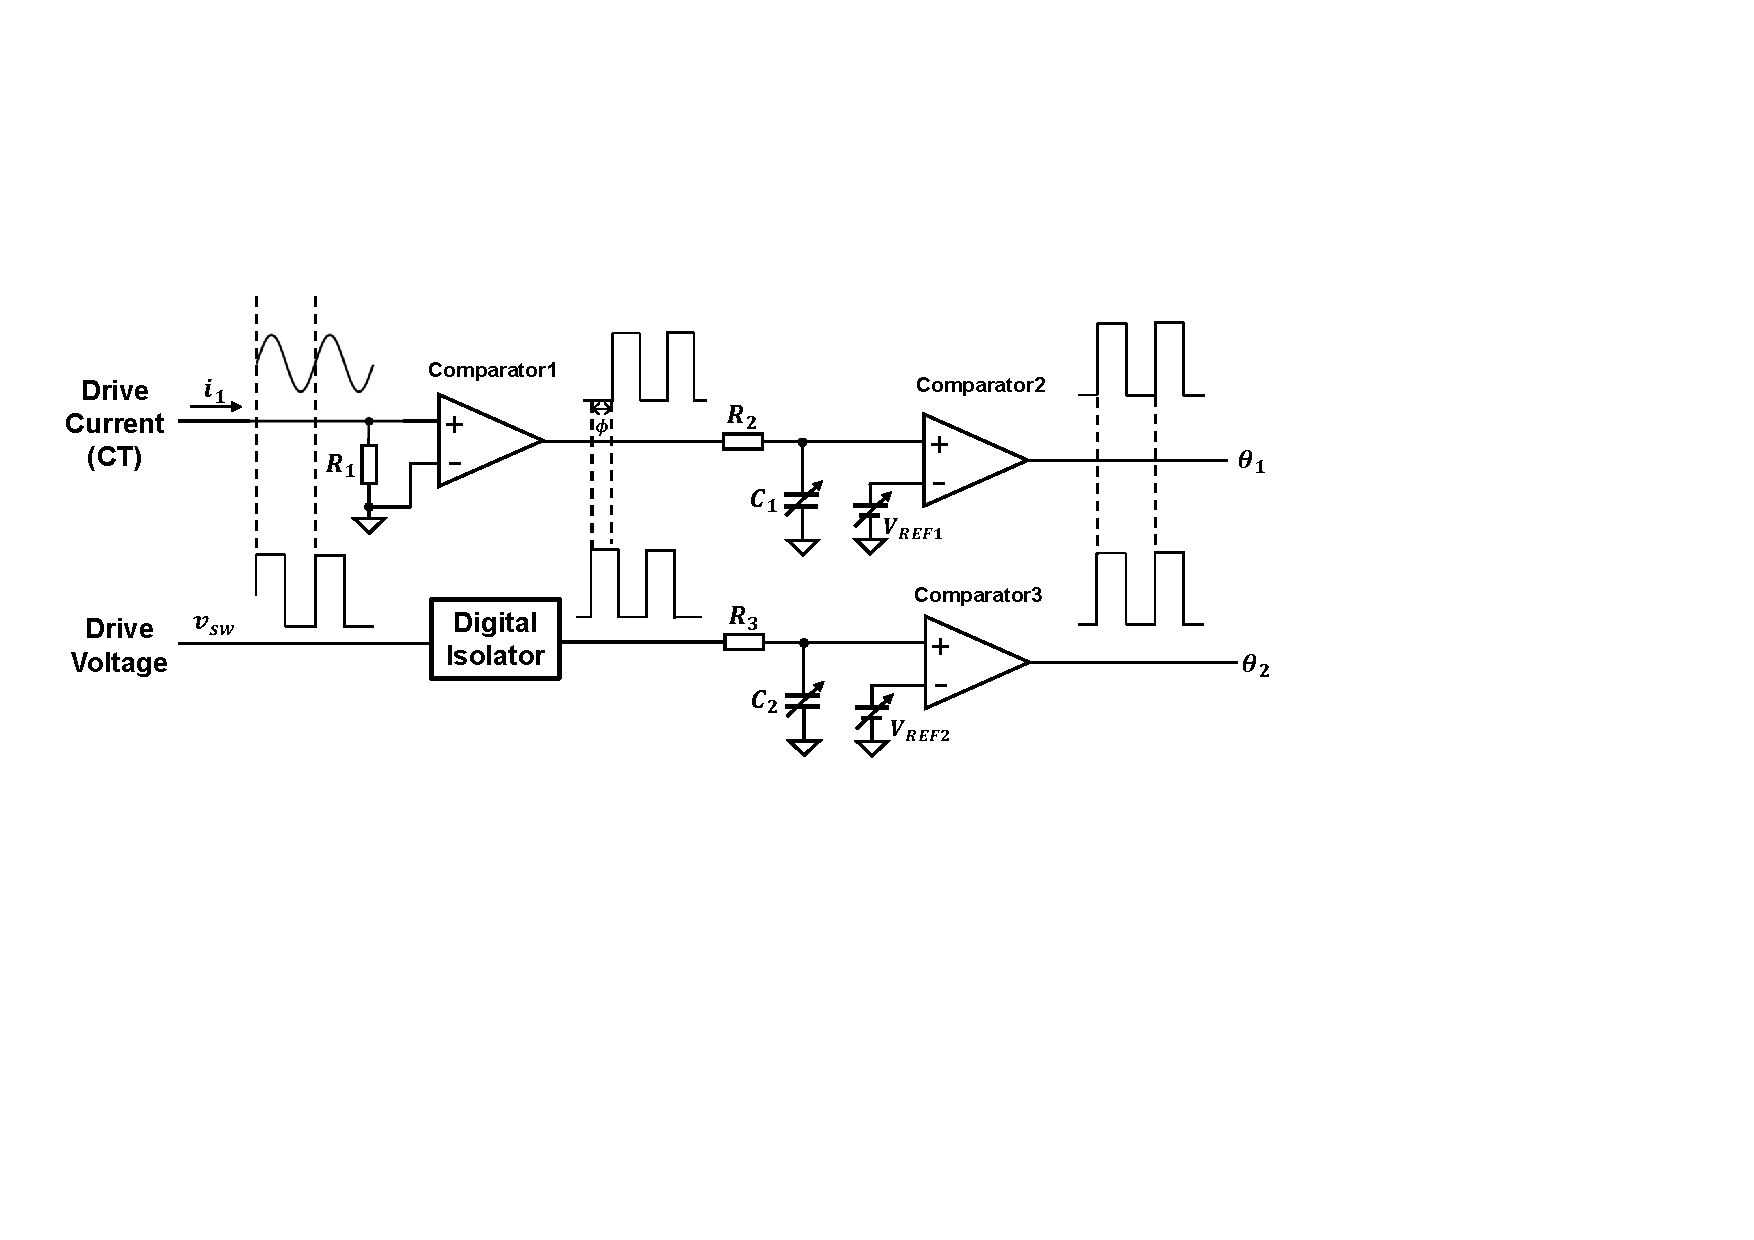
\includegraphics[width=160mm]{figures/delaycompensator.pdf}
\caption{波形整形・遅延補正回路}
\label{delaycompensator}

\end{center}
\end{figure}

\subsection{シミュレーション}
図\ref{pllsimulationcircuit}に,図\ref{entireblock}の構成による,PLLを用いたZRF自動追従回路のシミュレーション回路図を示す.なお,本稿における回路シミュレーションには,すべてLinear Technology社のLTspiceを用いている.ここで,伝送部のパラメータは表2.1の通りとし,伝送コイル間の相互インダクタンス$M$は$2.5 \, \mathrm{\mu H}$ (結合係数$k=0.5$)とした.また,PFDは文献\cite{Enzaka2014}や\cite{Razavi2004}で述べられている,2つのDフロップフロップならびに1つのANDゲートからなる構成とした.さらに,VCOには,$0-1 \, \mathrm{V}$の制御電圧に対して$0-1000 \, \mathrm{kHz}$の正弦波を出力する理想素子を用いた.

\begin{figure}[H]
\begin{center}

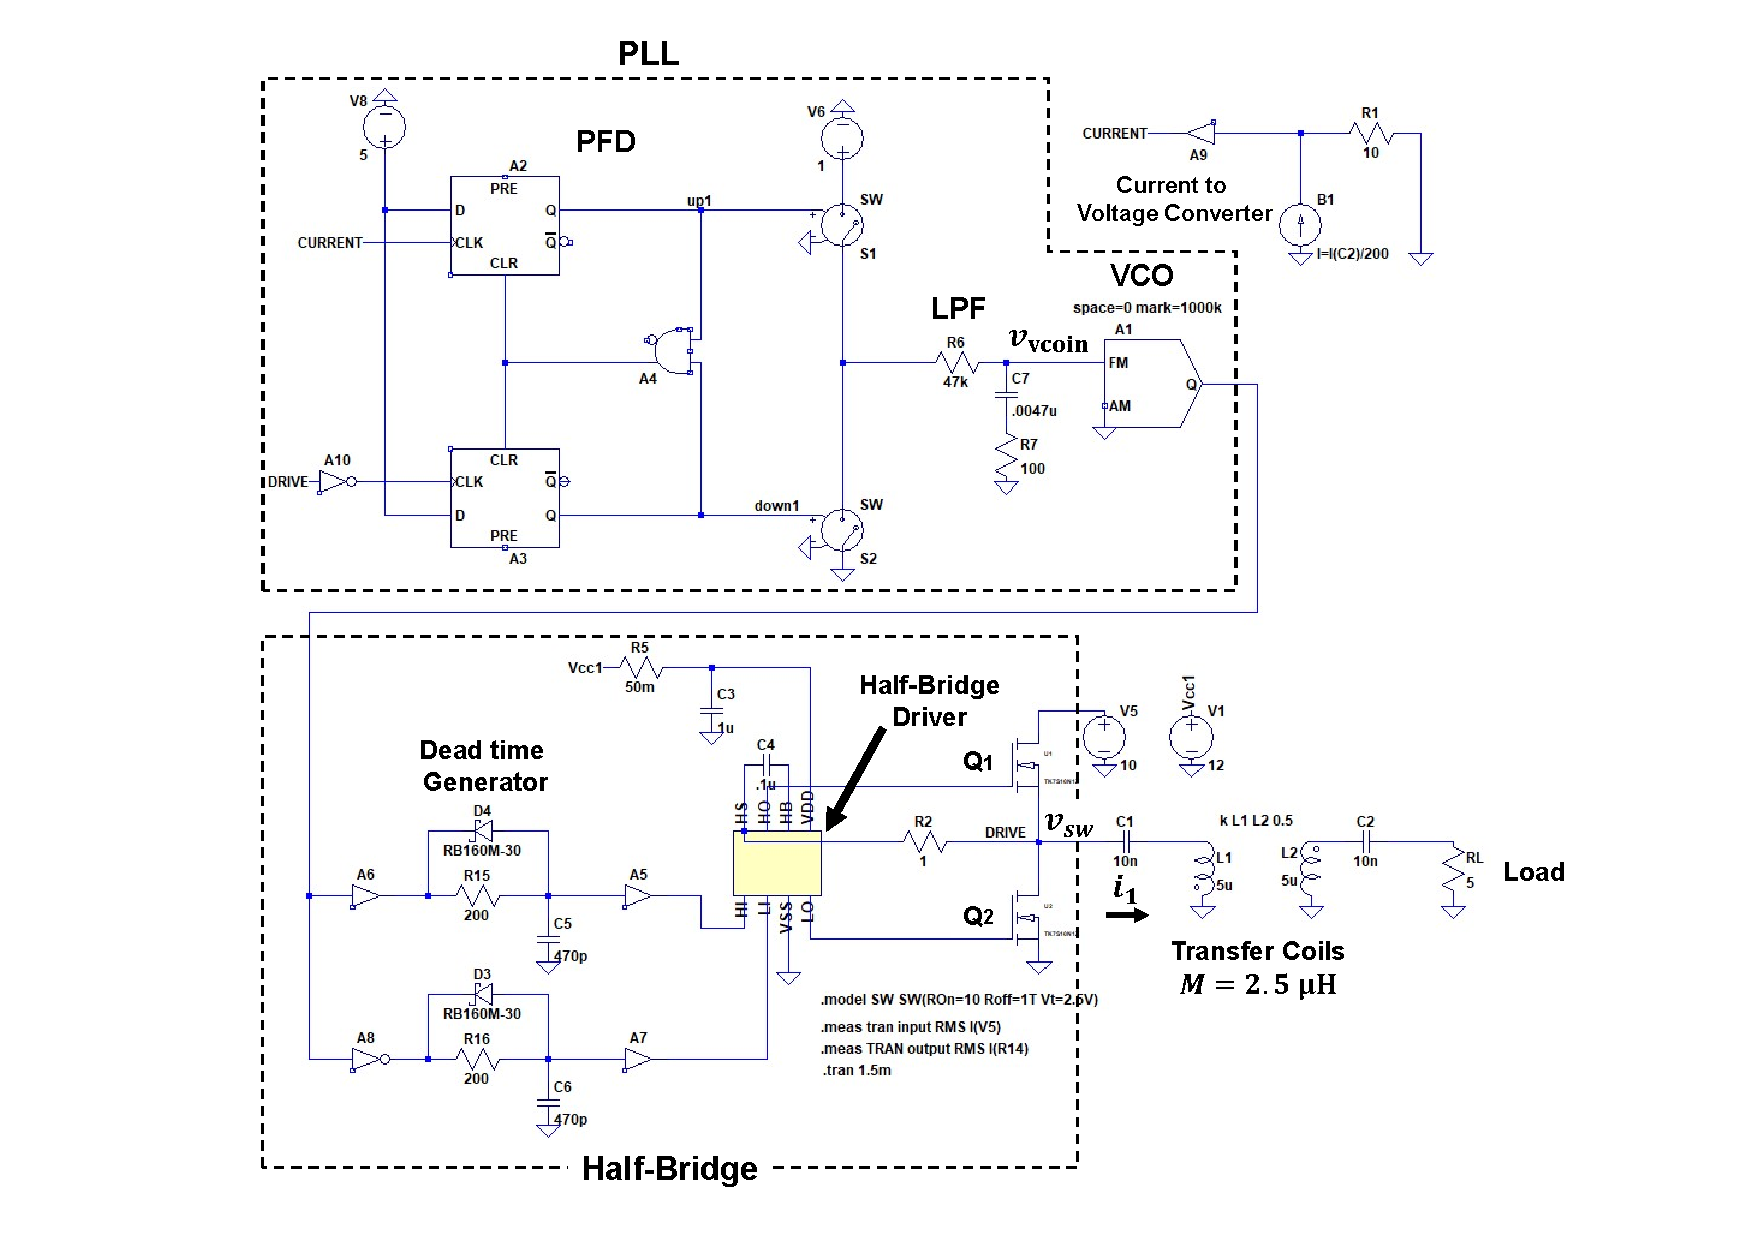
\includegraphics[width=145mm]{figures/pllsimulationcircuit.pdf}
\caption{ZRF追従のシミュレーション回路}
\label{pllsimulationcircuit}

\end{center}
\end{figure}

図\ref{pllsimulationgraph1}に,VCOの制御電圧$v_{vcoin}$の過渡解析結果を示す.$f_{ZRF1}$の理論値は,式(2.17)から約$597 \, \mathrm{kHz}$であり,このときの$v_{vcoin}$の理論値は$0.597 \, \mathrm{V}$である.図\ref{pllsimulationgraph1}より,$v_{vcoin}$は$0.597 \, \mathrm{V}$に漸近し,PLLが$f_{ZRF1}$にロックするよう動作していることが分かる.\par 
図\ref{pllsimulationgraph2}は,図\ref{pllsimulationcircuit}においてLPFとVCOとの間を開放し,VCOの制御電圧$v_{vcoin}$として$0-1 \, \mathrm{V}$で変化するランプ波形を入力して,$v_{vcoin}$と負荷抵抗$R_L$における瞬時電力との関係を図示したものである.同図より,$v_{vcoin}=0.597 \, \mathrm{V}$において,負荷における出力電力はほぼ最大値をとることがわかる.以上より,図\ref{entireblock}の構成で,ZRFを追従して大きな出力電力を得るシステムを構築できることがシミュレーションにより確認できた.
\begin{figure}[h]
\begin{center}

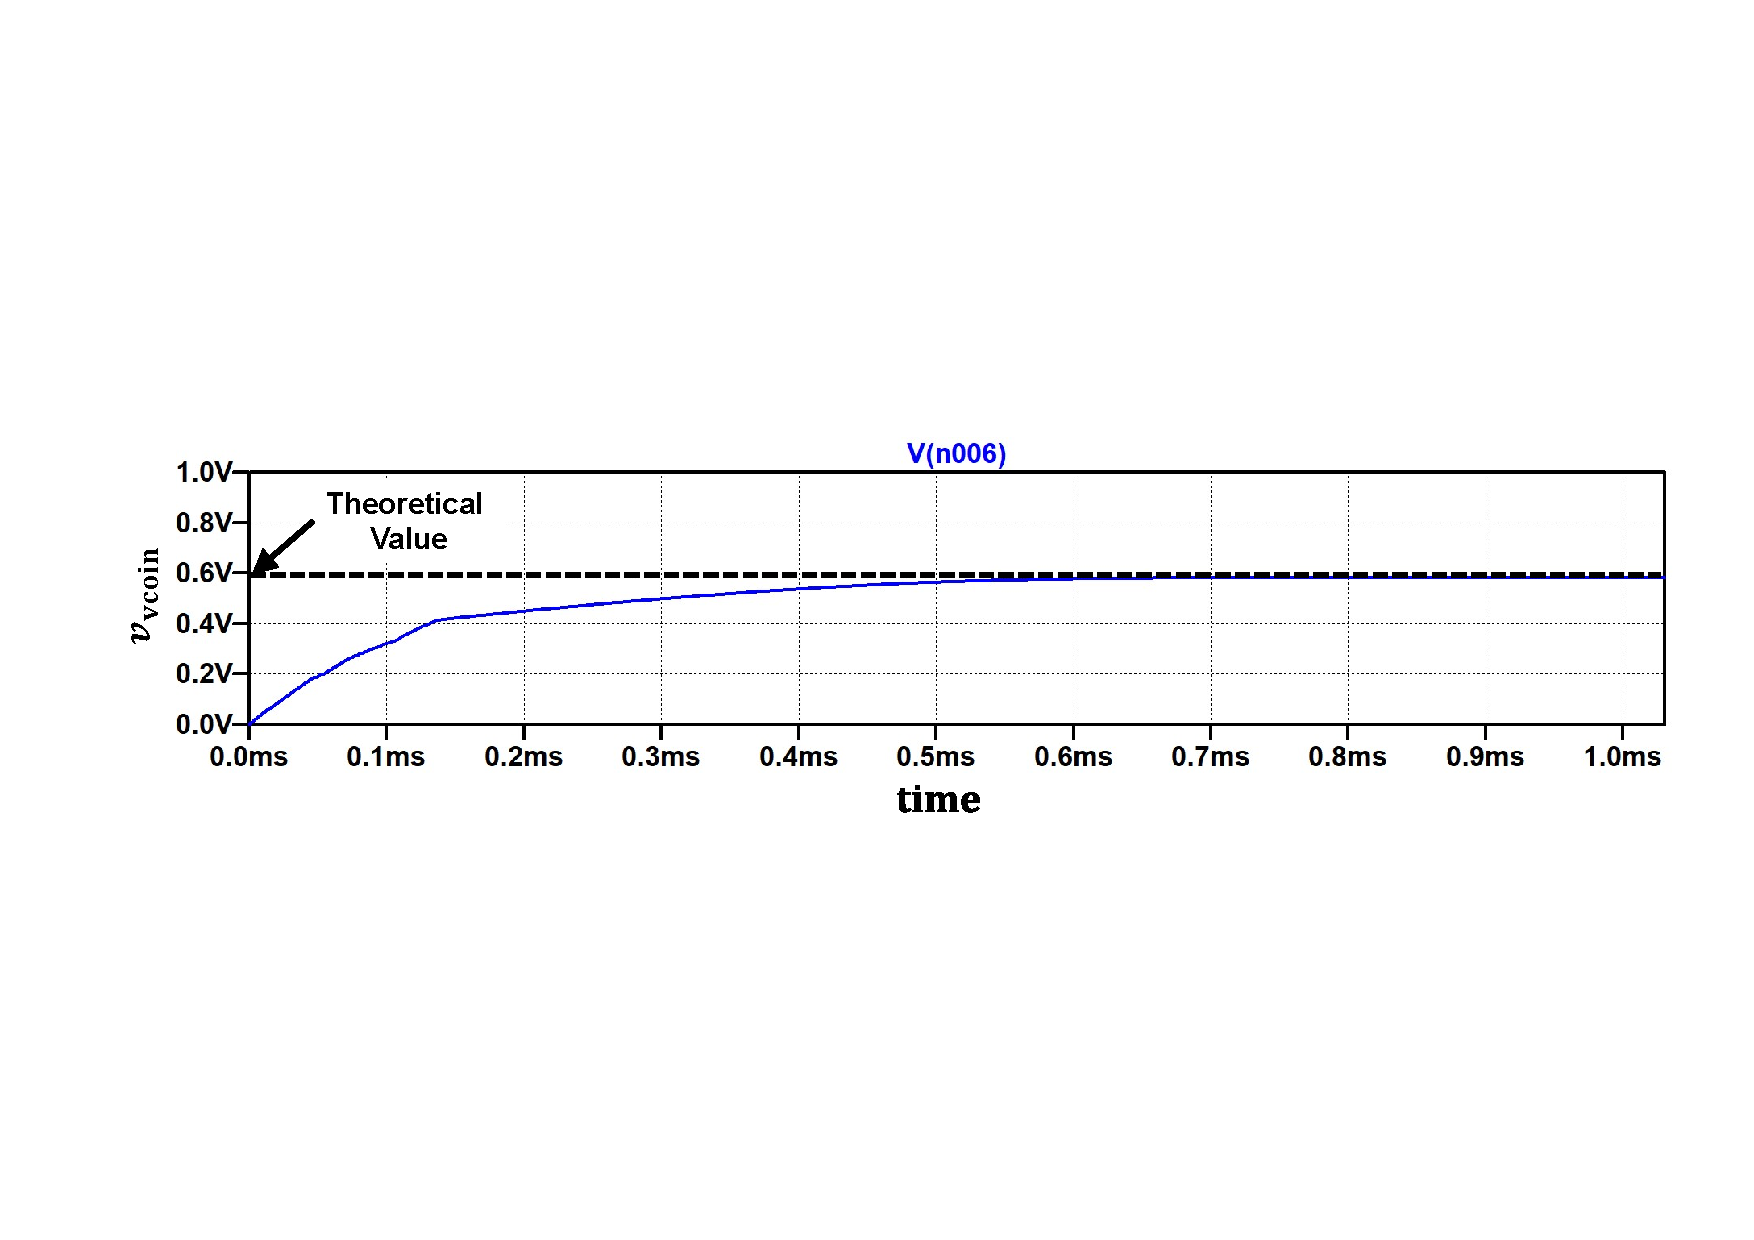
\includegraphics[width=150mm]{figures/pllsimulationgraph1.pdf}
\caption{VCO制御電圧の過渡解析結果}
\label{pllsimulationgraph1}

\vspace{1cm}

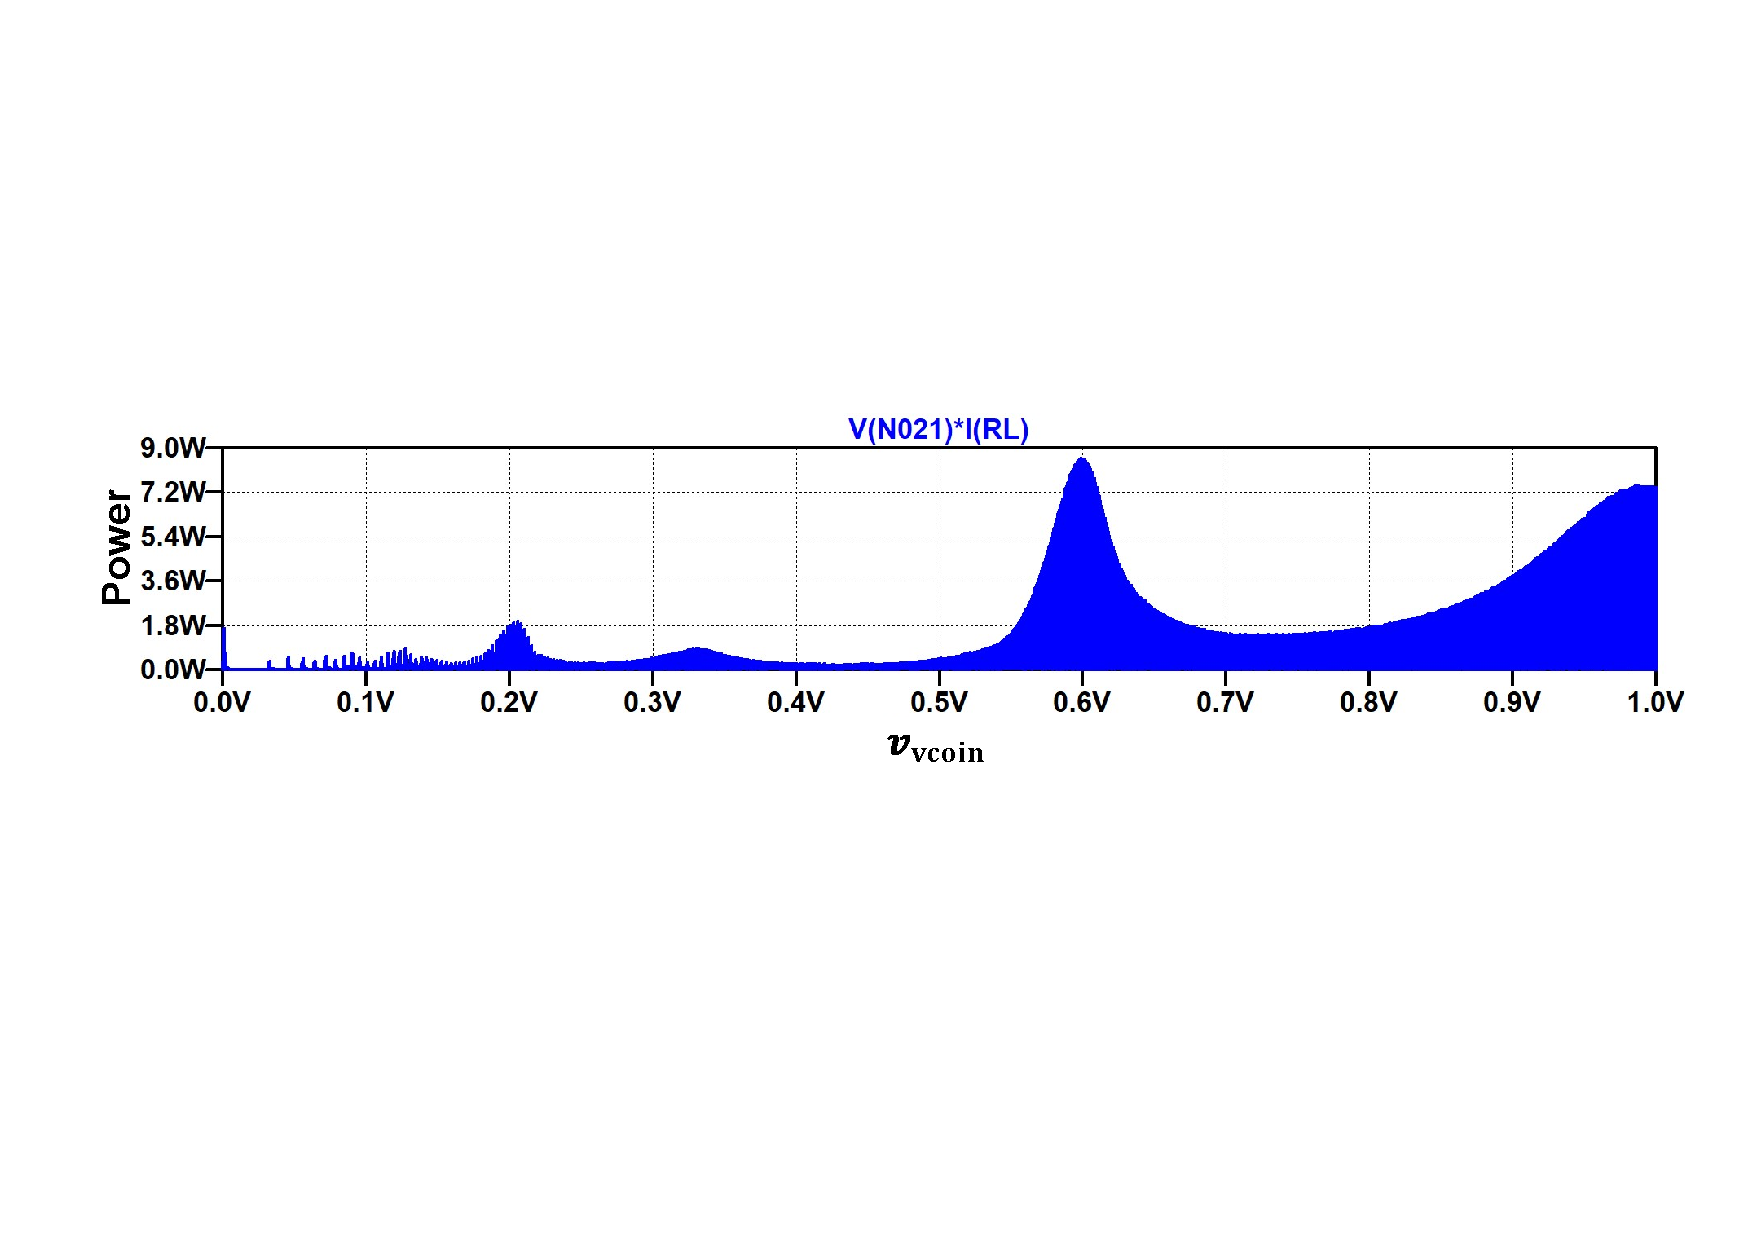
\includegraphics[width=150mm]{figures/pllsimulationgraph2.pdf}
\caption{VCO制御電圧と出力電力の関係}
\label{pllsimulationgraph2}

\end{center}
\end{figure}
